\chapter{Effects of alloying elements on the elastic properties of bcc ternary and higher ordered Ti-alloys}

\section{Introduction}

In order to develop a better understanding about alloying effect on the elastic properties of Ti alloys, the present work is developing an elastic database for the Ti-Mo-Nb-Sn-Ta-Zr system. With the focus being on bcc Ti-alloys, the effects of alloying elements on the pure elements and Ti-X binary alloys in the bcc phase were calculated in chapter 5. After extrapolating to higher order systems, it was hypothesized that studying the effects of alloying on the elastic properties of ternary alloys would improve the database. The present work focuses on studying the elastic properties of the Ti-X-Y (X $\neq$Y = Mo, Nb, Ta, Sn, and Zr) ternary alloys in the bcc phase. The single crystal elastic stiffness constants (c$_{ij}$'s) and polycrystalline aggregate properties are predicted across the composition range using Density Functional Theory (DFT) at 0 $^\circ$K outlined in the methodology chapter. Based on the DFT results, the CALPHAD approach outlined in the methodology is used to evaluate ternary interaction parameters. The interaction parameters are then incorporated into the database and the database accuracy is again tested similarily to the testing in chapter 5. The completed database is used to map the elastic modulus as a function of compostion. 

\section{Modeling and Calculations}

\subsection{Calculation details}

To study the elastic properties of the ternary bcc Ti alloys in the Ti-Mo-Nb-Sn-Ta-Zr system, DFT-based first-principles calculations were employed using the VASP (Vienna ab-initio simulation package) \cite{Kresse1996,Kresse1999}. Four kinds of calculations were performed for each ternary alloy Ti-X-Y, with the varying compositions of X$_{0.50}$Y$_{0.50}$ (16-atom supercell), Ti$_{0.33}$X$_{0.33}$Y$_{0.33}$ (36 atoms), Ti$_{0.50}$X$_{0.25}$Y$_{0.25}$ (32 atoms), Ti$_{0.74}$X$_{0.13}$Y$_{0.13}$ (64 atoms). The relaxation and use of SQS are discussed extensively in the methodology (chapter 2). The SQS used in this chapter were generated by Jiang et al. \cite{Jiang2004,Jiang2009}. The projector augmented wave (PAW) method was used to describe the ion-electron interaction. Based on our previous work done in chapter 5 (Figure \ref{Ch5-figure:PBEvsPW91}), the X-C functional of the generalized gradient approximation depicted by Perdew, Burke, and Ernzerhof (PBE-GGA) \cite{Perdew1996a} was employed. An energy cutoff roughly 1.3 times higher than the default values among all elements (i.e., 310 eV) was used for all calculations. The Brillouin zone sampling was done using the $\gamma$-centered Monkhorst-Pack scheme \cite{Monkhorst1976a}. The k-point grids used for the ternary SQS were 4x4x4 and the k-point grids used for the binary X$_{0.50}$Y$_{0.50}$ SQS structures were an automated k-point mesh generator in VASP with the length of the subdivision specified at 80. The elastic calculations were completed using a strain magnitude of $\pm$0.01 based on the study done in chapter 5 and the results seen in Figure \ref{Ch5-figure:Strain}.

\subsection{Modeling details}

The first-principles results were then used to model the ternary interaction parameters of the elastic stiffness constants. The modeling was completed by plotting the binary interpolation from the working database build in chapter 5. The plots started at a 50-50 mixture (X$_{0.50}$Y$_{0.50}$) of the alloying elements (X $\neq$ Y = Mo, Nb, Sn, Ta, and Zr) and plotted to pure Ti. The elastic stiffness constants of the pure elements and the binary interaction parameters from Table \ref{Ch5-table:tixelasip} were used to plot the binary interpolation. The differences between the ternary first-principles calculations and the binary interpolation were then used to obtain a single fitting parameter using the mathematica code in appendix C. With the focus being Ti-rich alloys and wanting to follow the same modeling technique used on the binary alloys, the first-principles results with 70 at.\% Ti or higher were weighted heavier (x6, according to the authors' practices) than the other points for the fittings. The best fit was found and the ternary interaction parameters were incorporated into the database. The databases was then used to predict the moduli values of the ternary and higher order alloys. 

\section{Results and discussion}

\subsection{Elastic calculation results}

The elastic stiffness coefficients $\overline{C}_{11}$, $\overline{C}_{12}$, and $\overline{C}_{44}$ are plotted in Figure \ref{Ch6-figure:tixyc11_1} to Figure \ref{Ch6-figure:tixyc44_2} for Ti-X-Y alloys (X $\neq$ Y = Mo, Nb, Sn, Ta, Zr). The plots start from a 50-50 mixture of the alloying elements X$_{0.50}$Y$_{0.50}$ to Ti. The calculations are plotted as circles, the interpolation from the pure elements and binary interaction parameters is plotted as a red dashed line. The difference between the calculations and binary interpolation was used to fit the ternary interaction parameters. The ternary fitting is plotted as a solid black line. The calculated elastic stiffness coefficients are listed in Table \ref{Ch6-table:tixyecijdata}.

The $\overline{C}_{11}$ values, for most of the Ti-X-Y systems, decrease from X$_{0.50}$Y$_{0.50}$ to Ti (see Figure \ref{Ch6-figure:tixyc11_1} and Figure \ref{Ch6-figure:tixyc11_2}). However, the Ti-Sn-Zr and Ti-Ta-Zr system differ. The $\overline{C}_{11}$ values, for the Ti-Sn-Zr (Figure \ref{Ch6-figure:tixyc11_2}d), first increase from Sn$_{0.50}$Zr$_{0.50}$ to 60 at. \% Ti and then decrease from 60 to 100 at. \% Ti. The $\overline{C}_{11}$ values, in the Ti-Ta-Zr system (Figure \ref{Ch6-figure:tixyc11_2}e), first increase from Ta$_{0.50}$Zr$_{0.50}$ to 35 at. \% Ti and then decrease from 35 to 100 at. \% Ti. The $\overline{C}_{12}$ results are plotted in Figure \ref{Ch6-figure:tixyc12_1} and Figure \ref{Ch6-figure:tixyc12_2}. The $\overline{C}_{12}$ values decrease from X$_{0.50}$Y$_{0.50}$ to Ti, for the Ti-Mo-Nb, Ti-Mo-Ta and Ti-Nb-Ta systems. The $\overline{C}_{12}$ values, for the Ti-Mo-Sn and Ti-Nb-Sn systems, first decrease from X$_{0.50}$Y$_{0.50}$ to 15 at. \% Ti then increase from 15 to 85 at. \% Ti and then decrease from 85 to 100 at. \% Ti. The Ti-Mo-Zr and Ti-Nb-Zr systems show a decrease in $\overline{C}_{12}$ value from X$_{0.50}$Y$_{0.50}$ to 60 at. \% Ti and then an increase from 60 to 100 at. \% Ti. The $\overline{C}_{12}$ values increase from X$_{0.50}$Y$_{0.50}$ to 70 at. \% Ti and then decrease from 70 to 100 at. \% Ti for the Ti-Sn-Ta system. For the Ti-Sn-Zr system, the values increase from 0 to 100 at. \% Ti and the $\overline{C}_{12}$ values, for the Ti-Ta-Zr system, first decrease from 0 to 70 at. \% Ti and then increase from 70 to 100 at. \% Ti. The $\overline{C}_{44}$ results are plotted in Figure \ref{Ch6-figure:tixyc44_1} and Figure \ref{Ch6-figure:tixyc44_2}. The The $\overline{C}_{44}$ values decrease from X$_{0.50}$Y$_{0.50}$ to Ti, for the Ti-Mo-Sn and Ti-Ta-Zr systems. For the Ti-Mo-Zr and Ti-Mo-Ta systems, the The $\overline{C}_{44}$ values first decrease from 0 to 80 at. \% Ti and then increase from 80 to 100 at. \% Ti. The The $\overline{C}_{44}$ values, for the Ti-Mo-Nb and Ti-Nb-Ta systems, first decrease from X$_{0.50}$Y$_{0.50}$ to 65 at. \% Ti and then increase from 65 to 100 at. \% Ti. The The $\overline{C}_{44}$ values first increase from 0 to 80 at. \% Ti and then decrease from 80 to 100 at. \% Ti for the Ti-Nb-Sn and Ti-Nb-Zr systems. For the Ti-Sn-Ta system (Figure \ref{Ch6-figure:tixyc44_2}c), the  values decrease from 0 until 20 at. \% Ti, then increase from 20 to 50 at. \% Ti and then decrease from 50 to 100 at. \% Ti. The The $\overline{C}_{44}$ values, for the Ti-Sn-Zr system, first increase from X$_{0.50}$Y$_{0.50}$ to 60 at. \% Ti and then decrease from 60 to 100 at. \% Ti.

The trends in the ternary elastic stiffness coefficients can be summarized and explained by looking at the elastic stiffness calculations done on the pure elements and Ti-X (X = Mo, Nb, Sn, Ta, Zr) in chapter 5. The c$_{11}$ and c$_{12}$ of Mo, Nb and Ta are higher than Ti, while Sn and Zr are lower. The c$_{44}$ for Mo and Ta are higher than Ti, while Nb, Sn, and Zr are lower. This can be explained because Mo, Nb and Ta are stable in the bcc structure at low temperatures while Ti, Sn and Zr are not, so the elastic stiffness coefficients are lower. The similarities of Mo, Nb and Ta are again noticed in the Ti-X data trends. The $\overline{C}_{11}$, $\overline{C}_{12}$, and $\overline{C}_{44}$ all follow the same trends for the Ti-Mo, Ti-Nb, and Ti-Ta systems with the $\overline{C}_{11}$ and $\overline{C}_{12}$ increasing in value from 100 to 0 at. \% Ti and the $\overline{C}_{44}$ decreasing and then increasing from 100 to 0 at. \% Ti. Based on this information, it is no surprise that the Ti-Mo-Nb, Ti-Mo-Ta and Ti-Nb-Ta systems have the same trends in their $c_{ij}$ data. When Ti-Mo, Ti-Nb, and Ti-Ta are alloyed with Sn in the ternary systems, they show similar trends for the most, not all, of the $c_{ij}$. The same is true for the Ti-Mo, Ti-Nb, and Ti-Ta systems alloyed with Zr.

Based on the discussion in the methodology, Born's criteria is used to look at the mechanical stability of the bcc phase. When $\overline{C}_{11}$-$\overline{C}_{12}$ becomes negative then the bcc phase loses mechanical stability and is thus plotted in Figure \ref{Ch6-figure:tixyc11-c12}. Based on the present results, the bcc phase loses mechanical stability in the Ti-Mo-Nb, Ti-Mo-Ta, Ti-Mo-Zr, Ti-Nb-Zr, Ti-Sn-Zr, and Ti-Ta-Zr systems when the Ti concentration is more than 90 at. \%, with the values being 91, 92, 95, 93, 91, and 94 at. \% Ti, respectively. The bcc phase loses mechanical stability at Ti concentrations above 87, 77, 89, and 80 at. \% Ti for Ti-Mo-Sn, Ti-Nb-Sn, Ti-Nb-Ta and Ti-Sn-Ta systems, respectively. Close to where the bcc phase loses its mechanical stability, the Young's modulus is reduced and such compositions may be desirable low modulus bcc Ti alloys. As discussed above, Mo, Nb and Ta are strong $\beta$-stabilizers and thus the Ti-Mo-Nb, Ti-Mo-Ta, and Ti-Nb-Ta systems stabilize the bcc phase similarly. Also, discussed previously, Zr is a weak $\beta$-stabilizer alone but when alloyed with other elements it acts a strong -stabilizer. This is observed with these results with the Ti-Mo-Zr, Ti-Nb-Zr, Ti-Ta-Zr systems all stabilizing the bcc phase at high Ti concentrations (95, 93, and 94 at. \% respectively). Zr is even able to stabilize the Ti-Sn-Zr system at a high Ti concentration of 91 at. \% Ti, even with Sn. Sn is not stable in the bcc phase and is not a -stabilizer. So, when alloyed with Sn, a higher concentration of other alloying elements is needed to stabilize the bcc phase. 

Figure \ref{Ch6-figure:tixyyoungs1} and Figure \ref{Ch6-figure:tixyyoungs2} plot the Young's moduli ($E$) calculations (circles) for each Ti-X-Y ternary system (X $\neq$ Y = Mo, Nb, Sn, Ta, Zr) starting from a 50-50 mixture of the two alloying elements to Ti. The red dashed line is the average from the Hill approach interpolated from the binary interaction parameters shown in Table \ref{Ch6-table:tixyelasip}. The average from the Hill approach (black solid line), Voigt (purple dotted line), Reuss (gold dotted-dashed line) bounds are plotted using the binary and ternary interaction parameters. The Voigt and Reuss bounds vary more drastically when the bcc structure is unstable as opposed to when the bcc structure is stable. The average  from the Hill approach using the binary and ternary interaction parameters is what the database predicts because it has been shown to be a more accurate representation of the Young's modulus than the Voigt or Reuss approximations \cite{Yue2009,Chung1967}. Whenever possible experimentally determined Young's moduli \cite{Niinomi2012,Mohammed2014,Nozoe2007,Geetha2009} (data listed in Table \ref{Ch6-table:tixyelasdata}) are plotted for comparison. The difference/error between the previous results (both experimental and from calculations) and the present first-principles results are calculated by Eq. \ref{eq: error}.

The first-principles $E$, for the Ti-Mo-Nb (Figure \ref{Ch6-figure:tixyyoungs1}a) system are compared with experimentally obtained $E$ data in the review paper by Niinomi et al. \cite{Niinomi2012}. The experimental $E$ results were obtained using a nanoindenter after solution treatment. The experimental $E$ values are higher than the Hill average calculated values (difference of 71 GPa or an error of 0.65 using Eq. \ref{eq: error}) and more closely match the Voigt bound (difference of 46 GPa). Niinomi \cite{Niinomi2012} pointed out that Young's moduli obtained from the microhardness testing are higher than the polycrystalline Young's moduli value, thus our calculation results should be close to the polycrystalline $E$ values. The present data show that the $E$ decreases in value from 0 to 100 at. \% Ti. 

In the literature, no bcc Ti-Mo-Sn (Figure \ref{Ch6-figure:tixyyoungs1}b) experimental $E$ results were found to be compared with the present work. The Voigt-Reuss bounds and the Hill average are quite similar until around 65 at. \% Ti when they begin to vary. The $E$ values decrease from 0 to 100 at. \% Ti. The calculated $E$ results for the Ti-Mo-Ta alloy system (Figure \ref{Ch6-figure:tixyyoungs2}c) are compared with experimental data reported by Niinomi et al. \cite{Niinomi2012}and Mohammed et al. \cite{Mohammed2014}. The $E$ values reported by Niinomi et al. \cite{Niinomi2012} were obtained using an ultrasonic measurement after the samples were solution treated. Niinomi et al. \cite{Niinomi2012} pointed out that $E$ values obtained using the ultrasonic method obtained normally fall in between the $E$ values determined using tensile testing or microhardness testing. Niinomi et al. \cite{Niinomi2012} also showed that when multiple authors test the same composition alloy using the ultrasonic technique their answers vary less drastically than when multiple authors test the same compositions using tensile or microhardness. The experimental $E$ fit well with the present Voigt bound (difference of 9 GPa) and had an error of 0.46 (Eq. \ref{eq: error}) from the Hill average (difference of 33 GPa). The $E$ values decrease from 0 to 100 at. \% Ti. 

The calculated $E$ of the Ti-Mo-Zr alloy system (Figure \ref{Ch6-figure:tixyyoungs1}d) is compared with experimental values reported by Mohammed et al. \cite{Mohammed2014}. The error in the experiments and methodology was not discussed. The experimental $E$ \cite{Mohammed2014} and the present $E$ (Hill average) vary by less than 6 GPa and the $E$ values decrease from 0 to 100 at. \% Ti. Experimentally determined Young's moduli results from Niinomi et al. \cite{Niinomi2012}, Mohammed et al. \cite{Mohammed2014}, and Nozoe et al. \cite{Nozoe2007} are compared with the present $E$ calculations for the Ti-Nb-Sn alloy system (Figure \ref{Ch6-figure:tixyyoungs1}e). The experimental $E$ results reported by Niinomi et al. \cite{Niinomi2012} were obtained through tensile testing of samples that were solution treated and cold rolled. Niinomi et al. showed that $E$ results at this specific composition varied by 10 GPa. The $E$ results reported by Niinomi et al. \cite{Niinomi2012} and Mohammed et al. \cite{Mohammed2014} differ from the Hill average by 9 and 15 GPa, respectively (an error of 0.28 using Eq. \ref{eq: error}). The $E$ results from Nozoe et al. \cite{Nozoe2007} differ by 10, 32 and 78 GPa from the Voigt, Hill and Reuss results, respectively, and have an error of 0.56 (Eq. \ref{eq: error}). However, Nozoe et al. reported that the samples formed the metastable $\omega$ phase. The $\omega$ phase is a metastable hexagonal phase (space group P6/mmm) with lattice parameters closely matching those of the bcc phase. Nozoe et al. \cite{Nozoe2007} also discussed how the aging of the Ti-Mo-Sn samples greatly affected the $E$. The $E$ values, for the Ti-Nb-Sn system, increase from 0 to 35 at. \%Ti and then decrease from 35 to 100 at. \% Ti. So overall the calculations satisfactorily predicted the Young's moduli of the Ti-Mo-Nb, Ti-Mo-Sn, Ti-Mo-Ta, Ti-Mo-Zr and Ti-Nb-Sn systems. 

Figure \ref{Ch6-figure:tixyyoungs2} continues to plot the $E$ of the Ti-X-Y ternary alloy systems. The first-principles $E$, for the Ti-Nb-Ta system, are compared with experimentally determined $E$ values reported by Mohammed et al. \cite{Mohammed2014} (Figure \ref{Ch6-figure:tixyyoungs2}a). At this composition, the Voigt and Reuss bounds are very close to the Hill average. Thus, while the experimental $E$ result fits closer to the Reuss bound (difference of 8 GPa), the experimental $E$ result only varies by 15 and 21 GPa from the Hill and Voigt results, respectively and has an error of 0.28 (Eq. \ref{eq: error}). Niinomi et al. \cite{Niinomi2012} reported $E$ values for the Ti-Nb-Ta system. However, the experimental values at the same compositions varied by more than 40 GPa and thus his results were not plotted for comparison here. The $E$ decreases in value from 0 to 100 at. \% Ti in the Ti-Nb-Ta ternary system. 

The first-principles $E$ results for the Ti-Nb-Zr (Figure \ref{Ch6-figure:tixyyoungs2}b) system are compared with experimentally determined $E$ results from Geetha et al. \cite{Geetha2009},  Mohammed et al. \cite{Mohammed2014}, and Niinomi et al. \cite{Niinomi2012}. The experimental $E$ results reported by Niinomi et al. \cite{Niinomi2012} are for the Ti-13Nb-13Zr and Ti-27Nb-8Zr alloys. The results for the Ti-13Nb-13Zr were obtained using both the ultrasonic and 3-point bending tests and varied by 50 GPa, while the Ti-27Nb-8Zr results were obtained using tensile testing and varied by 50 GPa. The experimentally determined $E$ results varied from the present Voigt, Hill and Reuss results by an average of 9, 2, and 14 GPa, respectively and has an error of 0.08 (Eq. \ref{eq: error}) from the Hill average. The $E$ values first increase from 0 to 70 at. \% Ti and then decrease from 70 to 100 at. \% Ti, for the Ti-Nb-Zr system. The Ti-Sn-Ta, Ti-Sn-Zr and Ti-Ta-Zr alloy systems did not have experimental data to be compared with and our results are shown in Figure \ref{Ch6-figure:tixyyoungs2}c, Figure \ref{Ch6-figure:tixyyoungs2}d, and Figure \ref{Ch6-figure:tixyyoungs2}e, respectively. For the Ti-Sn-Ta system, the $E$ values decrease from 0 to 100 at. \% Ti. The $E$ values, for the Ti-Sn-Zr system, first increase from 0 to 60 at. \% Ti and then decrease from 60 to 100 at. \% Ti. The $E$ values for the Ti-Ta-Zr system first decrease from 0 to 15 at. \% Ti, where the values begin to increase from 15 to 30 at. \% Ti and then decrease from 30 to 100 at. \% Ti. 

The first-principles calculations and the CALPHAD fittings are done using data obtained at 0 $^\circ$K while the experiments are obtained using polycrystalline samples at 300 $^\circ$K. Considering this and the fact that the experimental measured $E$ values vary at the same composition, the experimental values fit well within the bounds set by Reuss and Voigt, and the Hill average generally reproduces the experimentally determined $E$ data for the Ti-X-Y ternary alloys. 

Using the complete database with interaction parameters listed in Table \ref{Ch5-table:tixelasip}, the elastic stiffness coefficients can be predicted and then the moduli values can be calculated and mapped. Figure \ref{Ch6-figure:tixymap1} and Figure \ref{Ch6-figure:tixymap2} uses the global minimization tools in pycalphad \cite{Otis2017}to map the $E$ based on composition for Ti-X-Y ternaries. The ternary maps all have regions in the Ti rich corner that are light blue indicating that the Young's moduli are low enough to be in the target $E$ range. With this fact and the fact that six of the Ti-X-Y ternaries all stabilize the bcc phase above 90 at. \% Ti, the database points to multiple composition ranges that would yield possible implant materials. The pycalphad code and completed database used are in appendix D and E.

The $B$ and $G$ moduli calculated (circles) are plotted in Figures \ref{Ch6-figure:tixybulk1}-\ref{Ch6-figure:tixyshear2} for each Ti-X-Y (X $\neq$ Y = Mo, Nb, Sn, Ta, Zr) system starting from a 50-50 mixture of X and Y to Ti. The red dashed line is the Hill average interpolated from the binary interaction parameters shown in Table \ref{Ch6-table:tixyelasip}. The Hill average (black solid line), Voigt (purple dotted line), Reuss (gold dotted-dashed line) bounds are plotted using the binary and ternary interaction parameters and listed in Table \ref{Ch6-table:tixyelasdata}. The $B$ values, for all the Ti-X-Y ternaries except Ti-Nb-Sn, Ti-Sn-Ta and Ti-Sn-Zr decrease from 0 to 100 at. \% Ti, as shown in Figure \ref{Ch6-figure:tixybulk1} and Figure \ref{Ch6-figure:tixybulk2}. The $B$ values for the Ti-Nb-Sn and Ti-Sn-Ta systems first decrease from 0 to 10 at. \% Ti and then increase from 10 to 55 at. \% Ti and then decrease from 55 to 100 at. \% Ti. For the Ti-Sn-Zr system, the $B$ values first increase from 0 to 85 at. \% Ti and then decrease from 85 to 100 at. \% Ti. The $G$ values decrease from 0 to 100 at. \% Ti for all the ternary systems except Ti-Nb-Sn, Ti-Nb-Zr, Ti-Sn-Zr and Ti-Ta-Zr (Figure \ref{Ch6-figure:tixyshear1} and Figure \ref{Ch6-figure:tixyshear2}). The $G$ values increase from 0 to 60 at. \% Ti and then decrease from 60 to 100 at. \% Ti for the Ti-Nb-Sn, Ti-Nb-Zr systems. For the Ti-Sn-Zr system, the $G$ values first increase from 0 to 55 at. \% Ti and then decrease from 55 to 100 at. \% Ti. The $G$ values increase from 0 to 40 at. \% Ti and then decrease from 40 to 100 at. \% Ti for the Ti-Ta-Zr system. 


The $B$ and $G$ moduli calculated (circles) are plotted in Figure \ref{Ch6-figure:tixybulk1} to Figure \ref{Ch6-figure:tixyshear2} for each Ti-X-Y (X $\neq$ Y = Mo, Nb, Sn, Ta, Zr) system starting from a 50-50 mixture of X and Y to Ti. The red dashed line is the Hill average interpolated from the binary interaction parameters shown in Table \ref{Ch5-table:tixelasip}. The Hill average (black solid line), Voigt (purple dotted line), Reuss (gold dotted-dashed line) bounds are plotted using the binary and ternary interaction parameters (Table \ref{Ch5-table:tixelasip} and \ref{Ch6-table:tixyelasip}). The $B$ values, for all the Ti-X-Y ternaries except Ti-Nb-Sn, Ti-Sn-Ta and Ti-Sn-Zr decreases from 0 to 100 at.\% Ti, as shown in Figure \ref{Ch6-figure:tixybulk1} and Figure \ref{Ch6-figure:tixybulk2}. The $B$ values for the Ti-Nb-Sn and Ti-Sn-Ta systems first decrease from 0 to 10 at.\% Ti and then increase from 10 to 55 at.\% Ti and then decrease from 55 to 100 at.\% Ti. For the Ti-Sn-Zr system, the $B$ values first increase from 0 to 85 at.\% Ti and then decreases from 85 to 100 at.\% Ti. The $G$ values decrease from 0 to 100 at.\% Ti for all the ternary systems except Ti-Nb-Sn, Ti-Nb-Zr, Ti-Sn-Zr and Ti-Ta-Zr (Figure \ref{Ch6-figure:tixyshear1} and Figure \ref{Ch6-figure:tixyshear2}). The $G$ values increase from 0 to 60 at.\% Ti and then decrease from 60 to 100 at.\% Ti for the Ti-Nb-Sn, Ti-Nb-Zr systems. For the Ti-Sn-Zr system, the $G$ values first increase from 0 to 55 at.\% Ti and then decrease from 55 to 100 at.\% Ti. The $G$ values increase from 0 to 40 at.\% Ti and then decrease from 40 to 100 at.\% Ti for the Ti-Ta-Zr system. 

Both the $G$ and $E$ are negative when they are close to Ti. This is due to the instability of the bcc phase close to Ti. As discussed by Born’s criteria, when $\overline{C}_{11}$-$\overline{C}_{12}$ is negative the bcc phase loses mechanical stability. The Voigt bound of $G_{v}$ is expressed by:

%%
\begin{equation}
\label{eq: Gv}
G_v = \left( \overline{C}_{11}-\overline{C}_{12}+\overline{C}_{44} \right)/5
\end{equation}
%%

So, when $\overline{C}_{11}$-$\overline{C}_{12}$ is negative, it can cause $G$ to be negative. The $E$ is then calculated from the $B$ and $G$, so when $G$ is negative it can cause $E$ to be negative. This is one of the reasons that finding bcc Ti alloys close to the bcc stability will produce a low $E$. 



\subsection{Extrapolation to higher ordered systems}

The Young's moduli are predicted and compared with experimental results for higher order Ti alloys and the results are shown in Table \ref{Ch6-table:tixydatacomp} and Figure \ref{Ch6-figure:tixydatabase}. The same comparison was made in chapter 5, but those predictions were made without the ternary interaction parameters. Figure \ref{Ch6-figure:tixydatabase} plots the calculated Young's moduli (Hill average) versus the experimentally determined Young's moduli \cite{Tane2010a,Mohammed2014,Geetha2009}. The black diagonal line would be a perfect correlation between the predictions and experiments. The grey region is the average variance in the first-principles calculations when calculating the average elastic stiffness coefficients using Eq. \ref{eq: averagec11}-Eq. \ref{eq: averagec44} (3 GPa). The same higher order alloys were picked to compare the effect of introducing the ternary interaction parameters. As discussed previously, the error bars plotted for the experiments come from the variance that was seen when comparing the experimentally determined Young's moduli at the same composition from Niinomi et al. \cite{Niinomi2012}, Geetha et al. \cite{Geetha2009}, Tane et al. \cite{Tane2010a}, and Mohammed et al. \cite{Mohammed2014}. The horizontal error bars are the Voigt and Reuss bounds. Previously, without ternary interaction parameters, the predictions and experimental results varied anywhere between 0.69 and 14 GPa and on average by 7 GPa. The calculations are usually larger than the experimental values due to the temperature difference: the computed single crystal elastic stiffness coefficients are at 0 $^\circ$K, while the experiments on the polycrystalline samples are usually performed at 300 $^\circ$K. As expected, introducing ternary interaction parameters improves the database. The introduction of the ternary interaction parameters improved the predictions to vary anywhere from 0.39 to 13 GPa from the experimental values with an average variance of only 5 GPa. Thus, while the ternary interactions have small effects on the final results, the introduction of Ti-containing ternary interaction parameters still improves the predictions and the database is more accurate to predict the Young's moduli of higher order Ti alloys. 

\section{Conclusion}

The present study systematically calculated the elastic properties of the bcc Ti ternary alloys, including the elastic stiffness constants, bulk modulus, shear modulus, and Young's modulus. Five alloying elements, Mo, Nb, Sn, Ta and Zr were studied. The general CALPHAD modeling approach was used to fit ternary interaction parameters. From the elastic stiffness constant data, the Ti-X-Y (X $\neq$ Y = Mo, Nb, Ta) showed the same trends in the data. This is to be expected because Mo, Nb, and Ta are similar elements that are strong $\beta$-stabilizers and stable in the bcc phase at low temperatures. It was also seen that the Ti-X-Sn (X = Mo, Nb, Ta) alloys showed similar trends in the data for most of the elastic stiffness constants, so did the Ti-X-Zr (X = Mo, Nb, Ta) alloys. The present calculations showed that the bcc Ti-alloy was mechanically stabilized at compositions less than 91, 92, 95, 93, 91, 94, 87, 77, 89, and 80 at \% Ti for the Ti-Mo-Nb, Ti-Mo-Ta, Ti-Mo-Zr, Ti-Nb-Zr, Ti-Sn-Zr, Ti-Ta-Zr, Ti-Mo-Sn, Ti-Nb-Sn, Ti-Nb-Ta and Ti-Sn-Ta alloys, respectively. As discussed above, Mo, Nb and Ta are strong $\beta$-stabilizers and thus the Ti-Mo-Nb, Ti-Mo-Ta, and Ti-Nb-Ta systems stabilize the bcc phase similarly. Also, discussed previously, Zr is a weak $\beta$-stabilizer alone but when alloyed with other elements it acts a strong $\beta$-stabilizer. This was observed with the Ti-Mo-Zr, Ti-Nb-Zr, Ti-Ta-Zr systems all stabilizing the bcc phase at high Ti concentrations (95, 93, and 94 at.\% respectively). Zr was even able to stabilize the Ti-Sn-Zr system at a high Ti concentration of 91 at.\% Ti, even with Sn not being a $beta$-stabilizer or stable in the bcc phase. 

The pure element elastic results along with the binary and ternary interaction parameters were combined into a database file in appendix D. The database was used to map possible alloy compositions to find potential materials with a Young's modulus in the target range for biomedical load-bearing implants using the pycalphd code in appendix E. Overall, the introduction of the ternary interaction parameters improved the database's ability to predict the $E$ of higher order alloys by a small amount. The complete database satisfactorily predicts the elastic properties of higher order Ti-alloys and will help guide future research to develop low-modulus biocompatible Ti alloys.

\newpage
\begin{longtable}[H]{ c c c c c}
	\caption{First-principles calculations of the elastic stiffness constants} 	\label{Ch6-table:tixyecijdata} \\
	\hline
	Reference & Ti$_{1-bc}$X$_b$Y$_c$ & $\overline{C}_{11}$ & $\overline{C}_{11}$ & $\overline{C}_{11}$ \\
	\hline
	\endhead
	\hline
	\endfoot
	This work & Ti & 93 & 115 & 41 \\
	This work & Ti$_{0.74}$Mo$_{0.13}$Nb$_{0.13}$ & 155 & 121 $\pm$4 & 34 $\pm$4 \\
	This work & Ti$_{0.50}$Mo$_{0.25}$Nb$_{0.25}$ & 222 $\pm$3 & 129 $\pm$3 & 33 $\pm$3 \\
	This work & Ti$_{0.33}$Mo$_{0.33}$Nb$_{0.33}$ & 269 $\pm$5 & 134 $\pm$3 & 42 $\pm$4 \\
	This work & Mo$_{0.50}$Nb$_{0.50}$ & 414 $\pm$6 & 165 $\pm$3 & 68 \\
	This work & Ti$_{0.74}$Mo$_{0.13}$Sn$_{0.13}$ & 137 $\pm$15 & 121 $\pm$2 & 56 $\pm$13 \\
	This work & Ti$_{0.50}$Mo$_{0.25}$Sn$_{0.250}$ & 160 $\pm$3 & 130 $\pm$8 & 71 $\pm$2 \\
	This work & Ti$_{0.33}$Mo$_{0.33}$Sn$_{0.33}$ & 167 $\pm$8 & 133 $\pm$6 & 75 $\pm$2 \\
	This work & Mo$_{0.50}$Sn$_{0.50}$ & 192 $\pm$28 & 130 $\pm$36 & 40 $\pm$31 \\
	This work & Ti$_{0.74}$Mo$_{0.13}$Ta$_{0.13}$ & 153 $\pm$1 & 125 $\pm$4 & 38 $\pm$3 \\
	This work & Ti$_{0.50}$Mo$_{0.25}$Ta$_{0.25}$ & 222 $\pm$2 & 136 $\pm$1 & 45 $\pm$3 \\
	This work & Ti$_{0.33}$Mo$_{0.33}$Ta$_{0.33}$ & 263 $\pm$4 & 145 $\pm$6 & 49 $\pm$4 \\
	This work & Mo$_{0.50}$Ta$_{0.50}$ & 370 $\pm$13 & 163 $\pm$4 & 63 $\pm$4 \\
	This work & Ti$_{0.74}$Mo$_{0.13}$Zr$_{0.13}$ & 125 $\pm$1 & 109 $\pm$8 & 35 $\pm$1 \\
	This work & Ti$_{0.50}$Mo$_{0.25}$Zr$_{0.25}$ & 160 $\pm$1 & 116 $\pm$5 & 34 $\pm$2 \\
	This work & Ti$_{0.33}$Mo$_{0.33}$Zr$_{0.33}$ & 182 $\pm$1 & 116 $\pm$2 & 31 $\pm$8 \\
	This work & Mo$_{0.50}$Zr$_{0.50}$ & 231 $\pm$7 & 118 $\pm$5 & 33 $\pm$8 \\
	This work & Ti$_{0.74}$Nb$_{0.13}$Sn$_{0.13}$ & 115 $\pm$4 & 118 $\pm$3 & 55 \\
	This work & Ti$_{0.50}$Nb$_{0.25}$Sn$_{0.25}$ & 131 $\pm$9 & 121 $\pm$6 & 64 $\pm$3 \\
	This work & Ti$_{0.33}$Nb$_{0.33}$Sn$_{0.33}$ & 134 $\pm$2 & 122 $\pm$3 & 67 $\pm$6 \\
	This work & Nb$_{0.50}$Sn$_{0.50}$ & 132 $\pm$4 & 118 $\pm$8 & 56 $\pm$4 \\
	This work & Ti$_{0.74}$Nb$_{0.13}$Ta$_{0.13}$ & 130 $\pm$3 & 124 $\pm$4 & 37 $\pm$3 \\
	This work & Ti$_{0.50}$Nb$_{0.25}$Ta$_{0.25}$ & 182 $\pm$1 & 129 $\pm$4 & 43 $\pm$6 \\
	This work & Ti$_{0.33}$Nb$_{0.33}$Ta$_{0.33}$ & 208 & 135 $\pm$1 & 44 $\pm$1 \\
	This work & Nb$_{0.50}$Ta$_{0.50}$ & 260 $\pm$2 & 148 $\pm$3 & 47 $\pm$3 \\
	This work & Ti$_{0.74}$Nb$_{0.13}$Zr$_{0.13}$ & 101 $\pm$2 & 113 $\pm$4 & 32 $\pm$3\\
	This work & Ti$_{0.50}$Nb$_{0.25}$Zr$_{0.25}$ & 122 $\pm$1 & 113 $\pm$3 & 28 $\pm$3 \\
	This work & Ti$_{0.33}$Nb$_{0.33}$Zr$_{0.33}$ & 143 $\pm$2 & 107 $\pm$5 & 28 $\pm$3 \\
	This work & Nb$_{0.50}$Zr$_{0.50}$ & 154 $\pm$5 & 110 $\pm$3 & 15 $\pm$2 \\
	This work & Ti$_{0.74}$Sn$_{0.13}$Ta$_{0.13}$ & 115 $\pm$6 & 121 $\pm$4 & 60 $\pm$2 \\
	This work & Ti$_{0.50}$Sn$_{0.25}$Ta$_{0.25}$ & 138 $\pm$13 & 125 $\pm$4 & 75 $\pm$4 \\
	This work & Ti$_{0.33}$Sn$_{0.33}$Ta$_{0.33}$ & 138 $\pm$6 & 131 $\pm$8 & 78 $\pm$1 \\
	This work & Sn$_{0.50}$Ta$_{0.50}$ & 133 $\pm$8 & 130 $\pm$4 & 60 $\pm$4 \\
	This work & Ti$_{0.74}$Sn$_{0.13}$Zr$_{0.13}$ & 97 $\pm$5 & 111 $\pm$4 & 55 $\pm$2 \\
	This work & Ti$_{0.50}$Sn$_{0.25}$Zr$_{0.25}$ & 99 $\pm$12 & 103 $\pm$4 & 59 $\pm$7 \\
	This work & Ti$_{0.33}$Sn$_{0.33}$Zr$_{0.33}$ & 96 $\pm$7 & 98 $\pm$3 & 55 $\pm$3 \\
	This work & Sn$_{0.50}$Zr$_{0.50}$ & 85 $\pm$7 & 87 $\pm$9 & 42 $\pm$3 \\
	This work & Ti$_{0.74}$Ta$_{0.13}$Zr$_{0.13}$ & 136 $\pm$36 & 103 $\pm$21 & 44 $\pm$5 \\
	This work & Ti$_{0.50}$Ta$_{0.25}$Zr$_{0.25}$ & 130 $\pm$3 & 117 $\pm$4 & 42 $\pm$7 \\
	This work & Ti$_{0.33}$Ta$_{0.33}$Zr$_{0.33}$ & 148 $\pm$1 & 115 $\pm$2 & 44 $\pm$2 \\
	This work & Ta$_{0.50}$Zr$_{0.50}$ & 157 $\pm$2 & 123 $\pm$3 & 35 $\pm$3 \\
	\hline
\end{longtable}
%%%

\newpage
\begin{longtable}[H]{ c c c c c }
	\caption{First-principles calculations of the bulk modulus $B$, shear modulus $G$, and Young's modulus $E$ in GPa for different atomic percent compositions of the bcc Ti-X-Y ternary systems at 0 $^{\circ}$K as well as experimental data obtained for the Young's modulus at 300 $^{\circ}$K by the references stated.} 	\label{Ch6-table:tixyelasdata} \\
	\hline
	Reference & Ti$_{100-2b}$X$_b$Y$_b$ & $B$ &$G$ & $E$\\
	\hline
	\endhead
	\hline
	\endfoot
	This work & Ti & 108 & -12.91 & -40.34\\
	This work & TiMo$_{12.5}$Nb$_{12.5}$ & 132 $\pm$4 & 26 $\pm$4 & 73 $\pm$4\\
	This work & TiMo$_{25.0}$Nb$_{25.0}$ & 160 $\pm$3 & 38 $\pm$3 & 105 $\pm$3\\
	This work & TiMo$_{33.3}$Nb$_{33.3}$ & 179 $\pm$5 & 51 $\pm$5 & 139 $\pm$5\\
	This work & Mo$_{50}$Nb$_{50}$ & 248 $\pm$6 & 87 $\pm$6 & 233 $\pm$6\\
	Expt 300 K \cite{Niinomi2012} & TiMo$_{6}$Nb$_{2}$ & & & 110\\
	This work & TiMo$_{12.5}$Sn$_{12.5}$ & 126 $\pm$15 & 27 $\pm$15 & 75 +$\pm$15\\
	This work & TiMo$_{25.0}$Sn$_{25.0}$ & 140 $\pm$8 & 39 $\pm$8 & 106 $\pm$8\\
	This work & TiMo$_{33.3}$Sn$_{33.3}$ & 144 $\pm$8 & 42 $\pm$8 & 114 $\pm$8\\
	This work & Mo$_{50}$Sn$_{50}$ & 151 $\pm$36 & 36 $\pm$36 & 100 $\pm$36\\
	This work & TiMo$_{12.5}$Ta$_{12.5}$ & 134 $\pm$4 & 25 $\pm$4 & 72 $\pm$4\\
	This work & TiMo$_{25.0}$Ta$_{25.0}$ & 165 $\pm$2 & 44 $\pm$3 & 122 $\pm$3\\
	This work & TiMo$_{33.3}$Ta$_{33.3}$ & 184 $\pm$6 & 53 $\pm$6 & 145 $\pm$\\
	This work & Mo$_{50}$Ta$_{50}$ & 232 $\pm$13 & 77 $\pm$13 & 208 $\pm$13\\
	Expt 300 K \cite{Mohammed2014} & TiMo$_{7}$Ta$_{1}$ & & & 74\\
	Expt 300 K \cite{Niinomi2012}  & TiMo$_{7}$Ta$_{1}$ & & & 74\\
	This work & TiMo$_{12.5}$Zr$_{12.5}$ & 114 $\pm$8 & 20 $\pm$8 & 55 $\pm$8\\
	This work & TiMo$_{25.0}$Zr$_{25.0}$ & 131 $\pm$5 & 29 $\pm$5 & 80 $\pm$5\\
	This work & TiMo$_{33.3}$Zr$_{33.3}$ & 138 $\pm$2 & 32 $\pm$8 & 89 $\pm$8\\
	This work & Mo$_{50}$Zr$_{50}$ & 156 $\pm$7 & 41 $\pm$8 & 113 $\pm$8\\
	Expt 300 K \cite{Mohammed2014} & TiMo$_{7}$Zr$_{3}$ & & & 64\\
	This work & TiNb$_{12.5}$Sn$_{12.5}$ & 117 $\pm$4 & 14 $\pm$4 & 41 $\pm$4\\
	This work & TiNb$_{25.0}$Sn$_{25.0}$ & 124 $\pm$9 & 26 $\pm$9 & 72 $\pm$9\\
	This work & TiNb$_{33.3}$Sn$_{33.3}$ & 126 $\pm$6 & 28 $\pm$6 & 78 $\pm$6\\
	This work & Nb$_{50}$Sn$_{50}$ & 123 $\pm$8 & 26 $\pm$8 & 72 $\pm$8\\
	Expt 300 K \cite{Mohammed2014} & TiNb$_{22}$Sn$_{2}$ & & & 44\\
	Expt 300 K \cite{Niinomi2012} & TiNb$_{22}$Sn$_{2}$ & & & 50\\
	Expt 300 K \cite{Nozoe2007} & TiNb$_{9}$Sn$_{3}$ & & & 58\\
	This work & TiNb$_{12.5}$Ta$_{12.5}$ & 126 $\pm$4 & 15 $\pm$4 & 43 $\pm$4\\
	This work & TiNb$_{25.0}$Ta$_{25.0}$ & 147 $\pm$6 & 35 $\pm$6 & 98 $\pm$6\\
	This work & $_{33.3}$Ta$_{33.3}$ & 159 $\pm$1 & 41 $\pm$1 & 113 $\pm$1\\
	This work & Nb$_{50}$Ta$_{50}$ & 185 $\pm$3 & 50 $\pm$3 & 140 $\pm$3\\
	Expt 300 K \cite{Mohammed2014} & TiNb$_{10}$Ta$_{19}$ & & & 55\\
	This work & TiNb$_{12.5}$Zr$_{12.5}$ & 109 $\pm$4 & -2 $\pm$4 & -6 $\pm$4\\
	This work & TiNb$_{25.0}$Zr$_{25.0}$ & 116 $\pm$3 & 14 $\pm$3 & 40 $\pm$3\\
	This work & TiNb$_{33.3}$Zr$_{33.3}$ & 119 $\pm$5 & 23 $\pm$5 & 66 $\pm$5\\
	This work & Nb$_{50}$Zr$_{50}$ & 125 $\pm$5 & 17 $\pm$5 & 50 $\pm$5\\
	Expt 300 K \cite{Mohammed2014} & TiNb$_{8}$Zr$_{8}$ & & & 77\\
	Expt 300 K \cite{Mohammed2014} & TiNb$_{12}$Zr$_{9}$ & & & 14\\
	Expt 300 K \cite{Mohammed2014} & TiNb$_{11}$Zr$_{3}$ & & & 50\\
	Expt 300 K \cite{Niinomi2012} & TiNb$_{17}$Zr$_{5}$ & & & 78\\
	Expt 300 K \cite{Geetha2009} & TiNb$_{8}$Zr$_{8}$ & & & 81\\
	This work & TiSn$_{12.5}$Ta$_{12.5}$ & 119 $\pm$6 & 13 $\pm$6 & 39 $\pm$6\\
	This work & TiSn$_{25.0}$Ta$_{25.0}$ & 129 $\pm$13 & 31 $\pm$13 & 86 $\pm$13\\
	This work & TiSn$_{33.3}$Ta$_{33.3}$ & 133 $\pm$8 & 28 $\pm$8 & 79 $\pm$8\\
	This work & Sn$_{50}$Ta$_{50}$ & 131 $\pm$8 & 20 $\pm$8 & 57 $\pm$8\\
	This work & TiSn$_{12.5}$Zr$_{12.5}$ & 106 $\pm$5 & 4 $\pm$5 & 13 $\pm$5\\
	This work & TiSn$_{25.0}$Zr$_{25.0}$ & 102 $\pm$12 & 15 $\pm$12 & 42 $\pm$12\\
	This work & TiSn$_{33.3}$Zr$_{33.3}$ & 97 $\pm$7 & 15 $\pm$7 & 43 $\pm$7\\
	This work & Sn$_{50}$Zr$_{50}$ & 86 $\pm$9 & 11 $\pm$9 & 32 $\pm$9\\
	This work & TiTa$_{12.5}$Zr$_{12.5}$ & 114 $\pm$21 & 30 $\pm$21 & 82 $\pm$21\\
	This work & TiTa$_{25.0}$Zr$_{25.0}$ & 121 $\pm$4 & 20 $\pm$7 & 58 $\pm$7\\
	This work & TiTa$_{33.3}$Zr$_{33.3}$ & 126 $\pm$2 & 30 $\pm$2 & 83 $\pm$2\\
	This work & Ta$_{50}$Zr$_{50}$ & 134 $\pm$3 & 26 $\pm$3 & 74 $\pm$3\\
	\hline
\end{longtable}
%%%

\newpage
\begin{table}[H]
	\caption{Evaluated interactions parameters ($L_2$, Eq. \ref{eq: error}) for the elastic stiffness constants of the Ti-containing ternary alloys.}
	\centering
	\begin{tabular}{ c c c c c }
		\hline
		Alloy & Interaction Parameter & $\overline{C}_{11}$ & $\overline{C}_{12}$ & $\overline{C}_{44}$\\
		\hline
		Ti-Mo-Nb & $L_2$ & -29.97 & 13.97 & 9.72\\
		Ti-Mo-Sn & $L_2$ & -83.85 & 31.80 & 74.73\\
		Ti-Mo-Ta & $L_2$ & -106.53 & -12.35 & 5.27\\
		Ti-Mo-Zr & $L_2$ & -245.27 & 50.43 & -44.96\\
		Ti-Nb-Sn & $L_2$ & -41.52 & 25.52 & 67.85\\
		Ti-Nb-Ta & $L_2$ & -93.77 & -15.80 & 4.25\\
		Ti-Nb-Zr & $L_2$ & -220.35 & 72.10 & -55.29\\
		Ti-Sn-Ta & $L_2$ & -95.39 & -10.94 & 67.85\\
		Ti-Sn-Zr & $L_2$ &  -155.34 & 68.86 & 3.85\\
		Ti-Ta-Zr & $L_2$ & -149.67 & -8.91 & -23.70\\		
		\hline
	\end{tabular}
	\label{Ch6-table:tixyelasip}
\end{table}
\clearpage
%%%


\newpage
\begin{table}[H]
	\caption{Predicted Young's moduli ($E$) (in GPa) of higher order alloys using the binary and ternary interaction parameters in the bcc phase compared to the predicted Young's moduli ($E_{BIN}$) using just the binary interaction parameters and the experimental values found with both the weight percent and atomic percent listed.}
	\centering
	\begin{tabular}{ c c c c c }
		\hline
		Alloy Name ($\%$wt) & at \% & Calc $E_{BIN}$ & Calc $E$ & Expt $E$\\
		\hline
		Ti-35Nb-7Zr-5Ta \cite{Geetha2009} & Ti-24Nb-5Zr-2Ta & 81 & 78 & 80\\
		Ti-29Nb-13Ta-4.6Zr \cite{Geetha2009}  & Ti-20Nb-5Ta-3Zr & 76 & 73 & 75\\
		Ti-29Nb-13Ta-6Sn \cite{Geetha2009} & Ti-21Nb-5Ta-3Sn & 68 & 68 & 74\\
		Ti-29Nb-13Ta-4.6Sn \cite{Geetha2009} & Ti-20Nb-5Ta-3Sn & 67 & 66 & 66\\
		Ti-29Nb-13Ta-4.5Zr \cite{Geetha2009} & Ti-20Nb-5Ta-3Zr & 76 & 73 & 65\\
		Ti-29Nb-13Ta-4.6Zr \cite{Tane2010a} & Ti-21Nb-5Ta-3Zr & 76 & 75 & 64\\
		Ti-30Nb-10Ta-5Zr \cite{Tane2010a} & Ti-23Nb-4Ta-3Zr & 77 & 74 & 64\\
		Ti-35Nb-10Ta-5Zr \cite{Tane2010a} & Ti-25Nb-4Ta-4Zr & 80 & 78 & 65\\
		Ti-24Nb-4Zr-7.9Sn \cite{Mohammed2014} & Ti-15Nb-3Zr-4Sn & 65 & 62 & 54\\
		Ti–35Nb–2Ta–3Zr \cite{Mohammed2014} & Ti-23Nb-1Ta-2Zr & 69 & 68 & 61\\
		Ti-29Nb-11Ta-5Zr \cite{Mohammed2014} & Ti-20Nb-6Ta-2Zr & 74 & 72 & 60\\
		Ti-10Zr-5Ta-5Nb \cite{Mohammed2014} & Ti-6Zr-1Ta-3Nb & 64 & 62 & 52\\
		Ti-29Nb-13Ta-2Sn \cite{Mohammed2014} & Ti-20Nb-5Ta-1Sn & 66 & 65 & 62\\
		\hline
	\end{tabular}
	\label{Ch6-table:tixydatacomp}
\end{table}
\clearpage
%%%

\pagebreak
\begin{figure}[H]
	\centering
	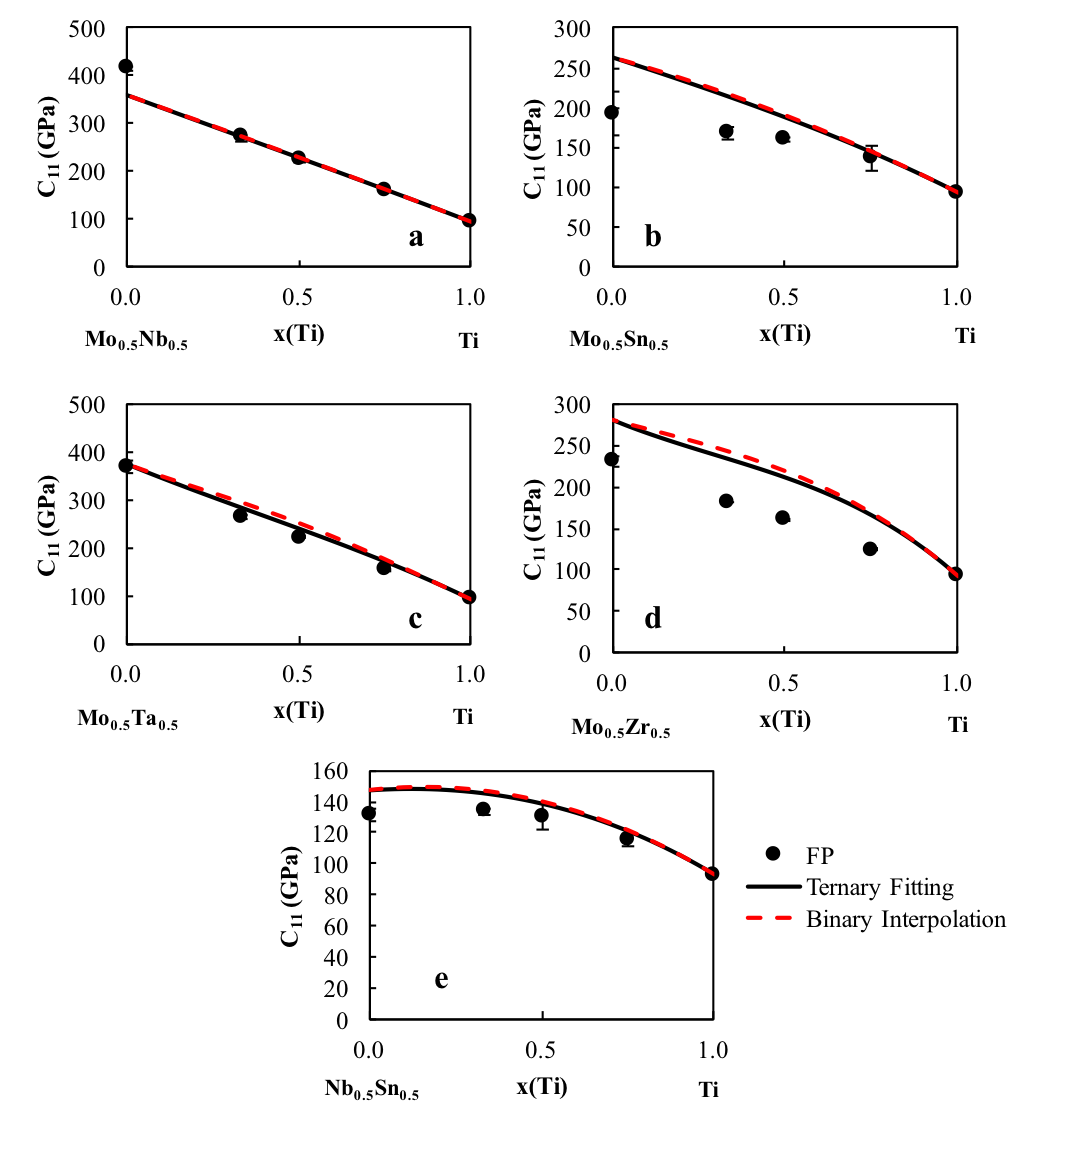
\includegraphics[width=\textwidth]{Chapter-6/Figures/tixyc111.png}
	\caption{Calculated $\overline{C}_{11}$ values (circles) plotted with their errors as well as the interpolation from the binary interaction parameters (red dashed line) and the ternary fitting (black dashed line) for five of the Ti-X-Y binary systems from a 50-50 mixture of the alloying elements X and Y to Ti (X $\neq$ Y = Mo, Nb, Ta, Sn, Zr).}
	\label{Ch6-figure:tixyc11_1}
\end{figure}

\pagebreak
\begin{figure}[H]
	\centering
	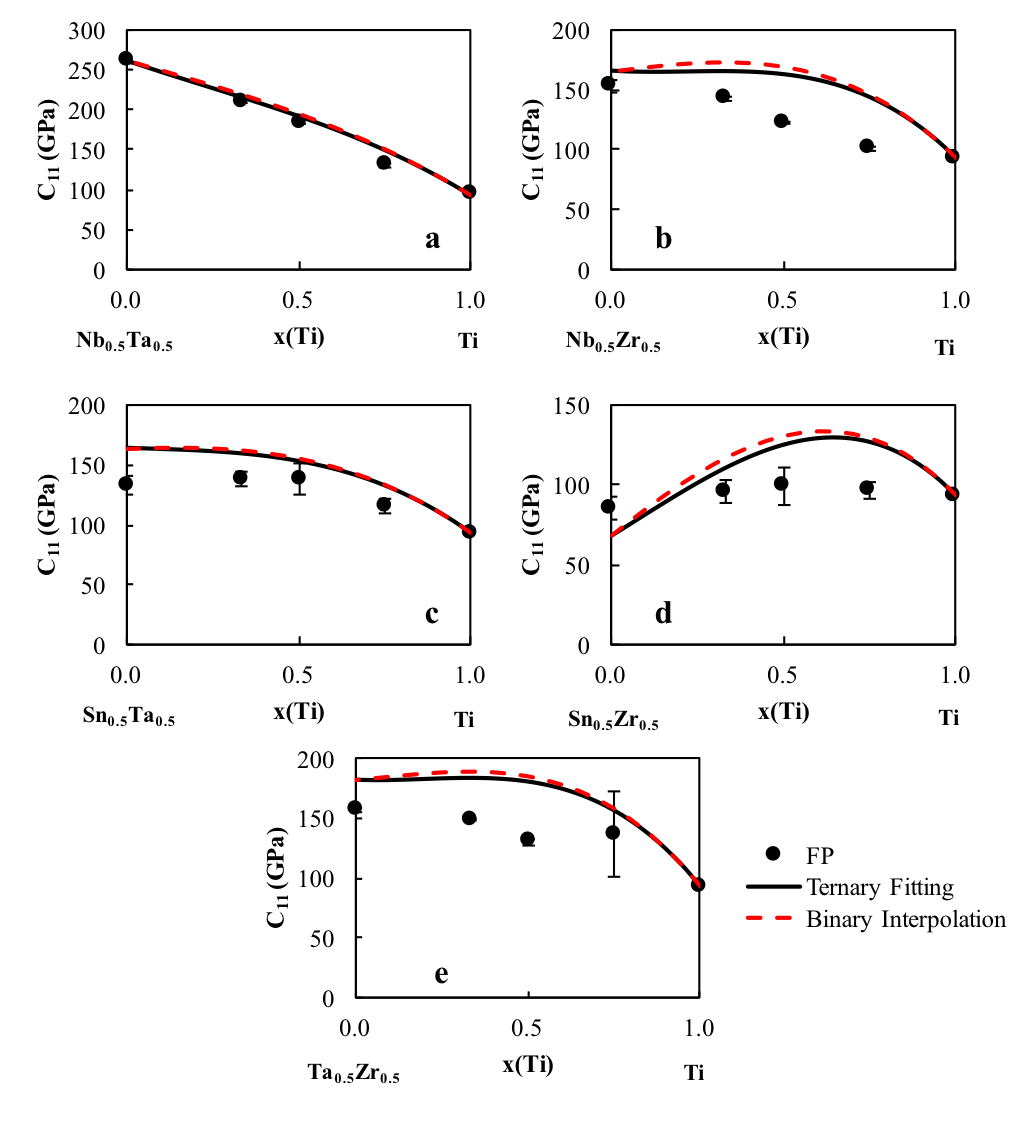
\includegraphics[width=\textwidth]{Chapter-6/Figures/tixyc112.png}
	\caption{Calculated $\overline{C}_{11}$ values (circles) plotted with their errors as well as the interpolation from the binary interaction parameters (red dashed line) and the ternary fitting (black dashed line) for five of the Ti-X-Y binary systems from a 50-50 mixture of the alloying elements X and Y to Ti (X $\neq$ Y = Mo, Nb, Ta, Sn, Zr).}
	\label{Ch6-figure:tixyc11_2}
\end{figure}


\pagebreak
\begin{figure}[H]
	\centering
	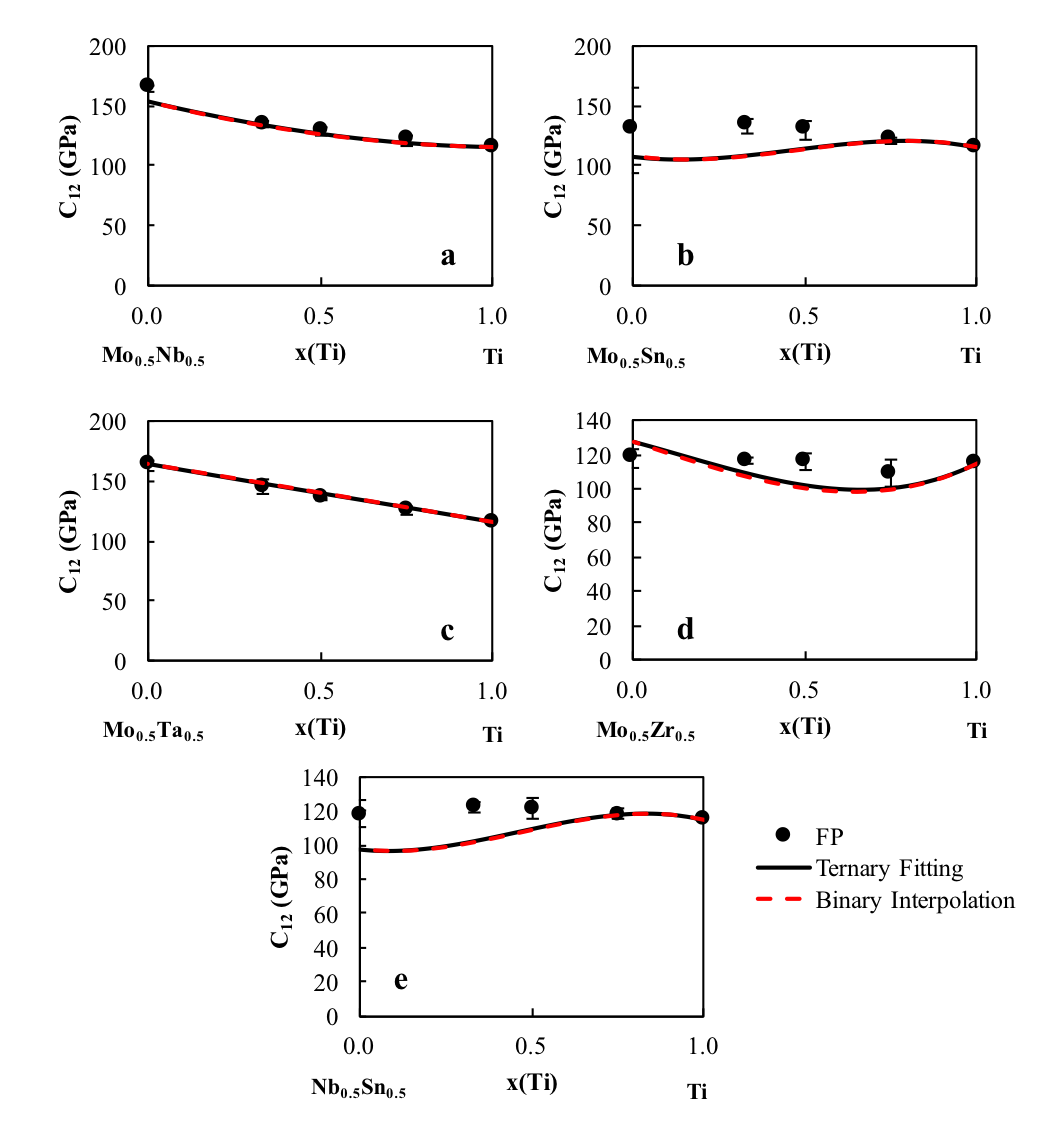
\includegraphics[width=\textwidth]{Chapter-6/Figures/tixyc121.png}
	\caption{Calculated $\overline{C}_{12}$ values (circles) plotted with their errors as well as the interpolation from the binary interaction parameters (red dashed line) and the ternary fitting (black dashed line) for five of the Ti-X-Y binary systems from a 50-50 mixture of the alloying elements X and Y to Ti (X $\neq$ Y = Mo, Nb, Ta, Sn, Zr).}
	\label{Ch6-figure:tixyc12_1}
\end{figure}

\pagebreak
\begin{figure}[H]
	\centering
	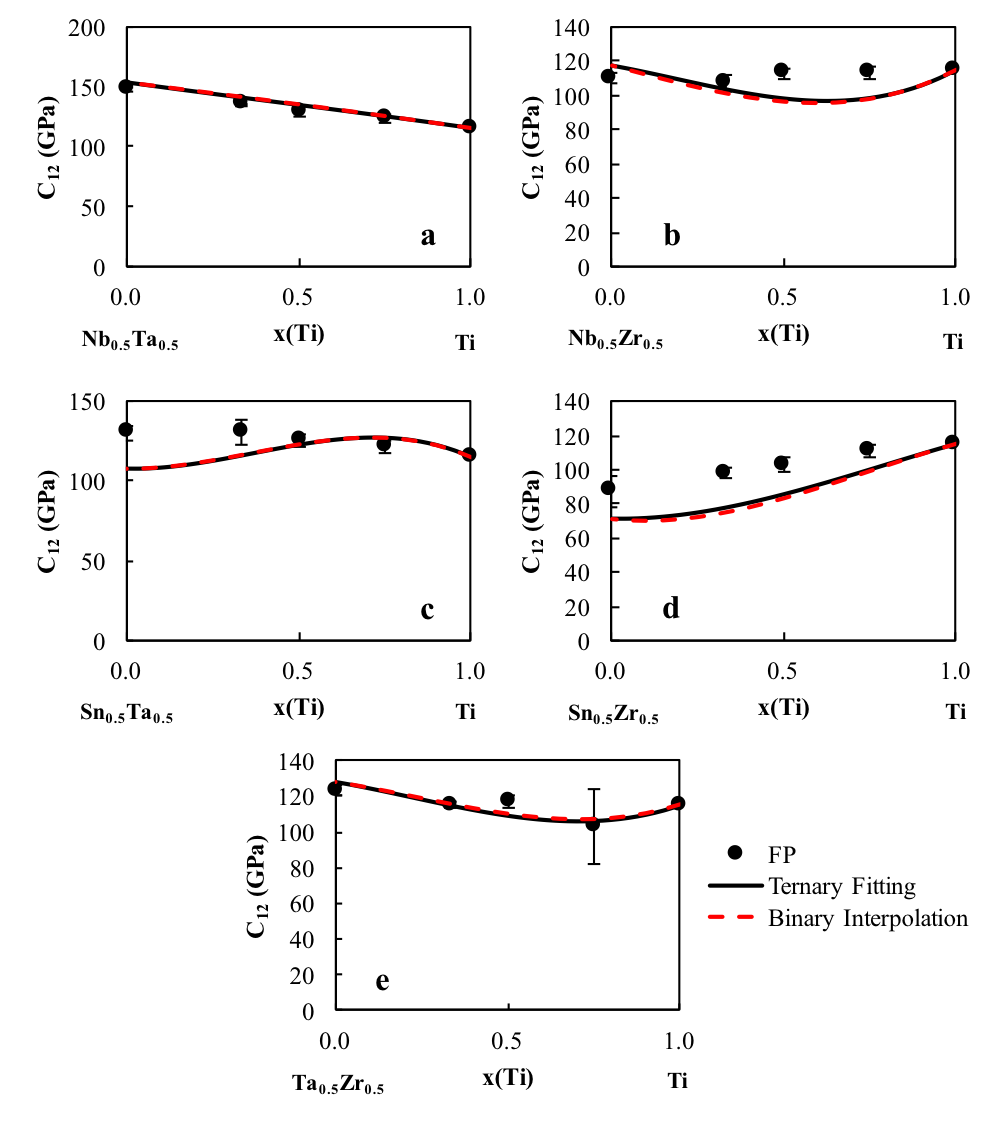
\includegraphics[width=\textwidth]{Chapter-6/Figures/tixyc122.png}
	\caption{Calculated $\overline{C}_{12}$ values (circles) plotted with their errors as well as the interpolation from the binary interaction parameters (red dashed line) and the ternary fitting (black dashed line) for five of the Ti-X-Y binary systems from a 50-50 mixture of the alloying elements X and Y to Ti (X $\neq$ Y = Mo, Nb, Ta, Sn, Zr).}
	\label{Ch6-figure:tixyc12_2}
\end{figure}

\pagebreak
\begin{figure}[H]
	\centering
	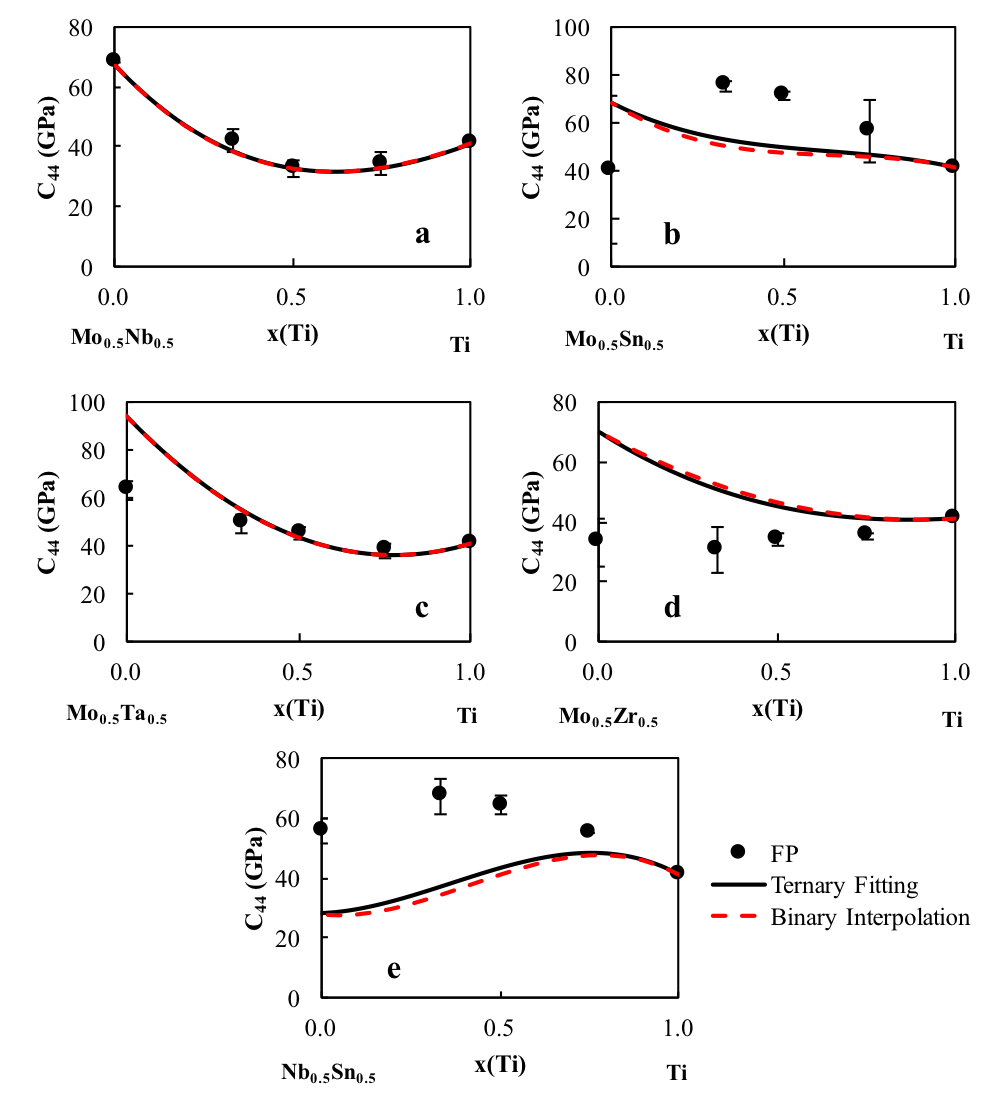
\includegraphics[width=\textwidth]{Chapter-6/Figures/tixyc441.png}
	\caption{Calculated $\overline{C}_{44}$ values (circles) plotted with their errors as well as the interpolation from the binary interaction parameters (red dashed line) and the ternary fitting (black dashed line) for five of the Ti-X-Y binary systems from a 50-50 mixture of the alloying elements X and Y to Ti (X $\neq$ Y = Mo, Nb, Ta, Sn, Zr).}
	\label{Ch6-figure:tixyc44_1}
\end{figure}

\pagebreak
\begin{figure}[H]
	\centering
	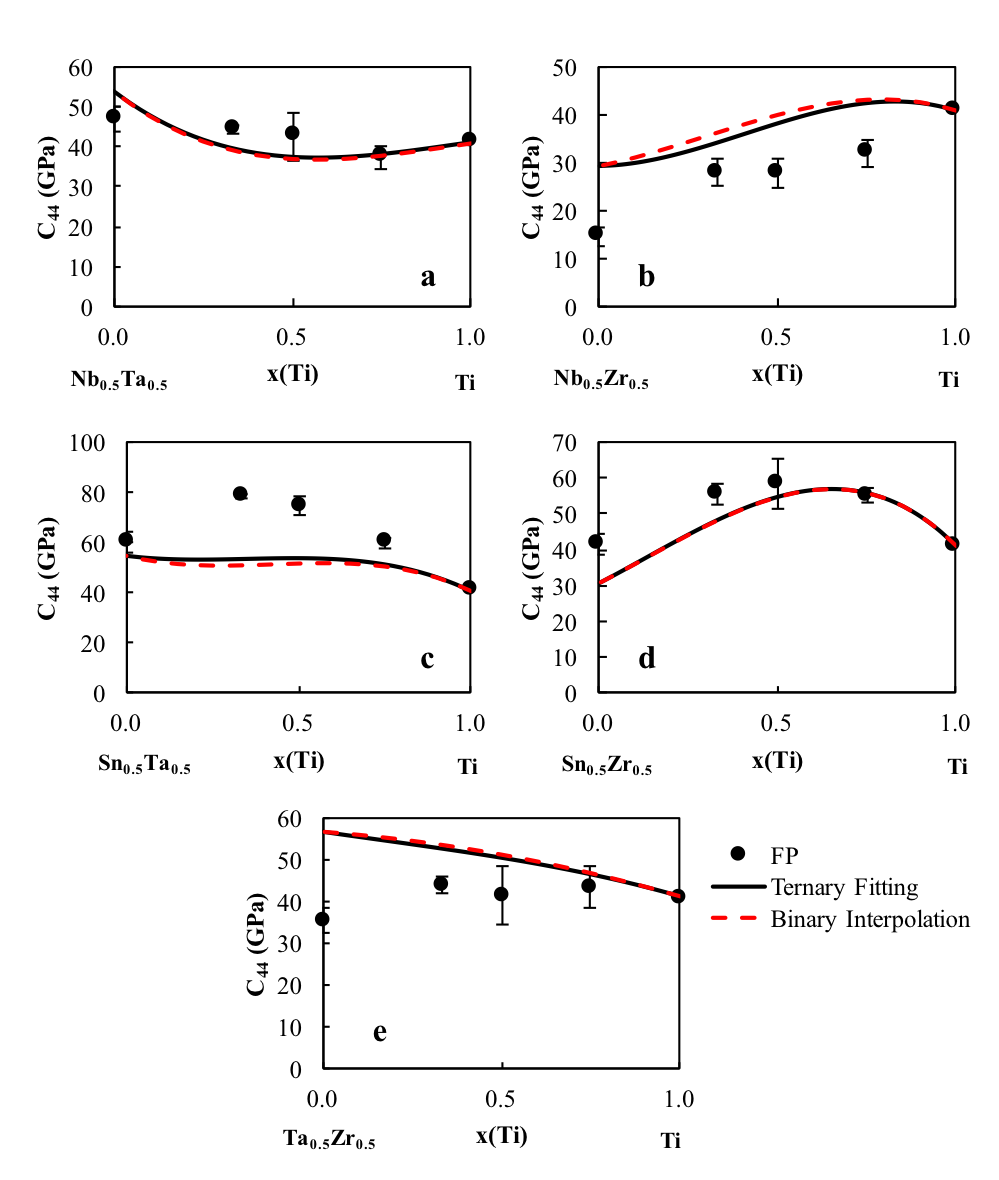
\includegraphics[width=\textwidth]{Chapter-6/Figures/tixyc442.png}
	\caption{Calculated $\overline{C}_{44}$ values (circles) plotted with their errors as well as the interpolation from the binary interaction parameters (red dashed line) and the ternary fitting (black dashed line) for five of the Ti-X-Y binary systems from a 50-50 mixture of the alloying elements X and Y to Ti (X $\neq$ Y = Mo, Nb, Ta, Sn, Zr).}
	\label{Ch6-figure:tixyc44_2}
\end{figure}

\pagebreak
\begin{figure}[H]
	\centering
	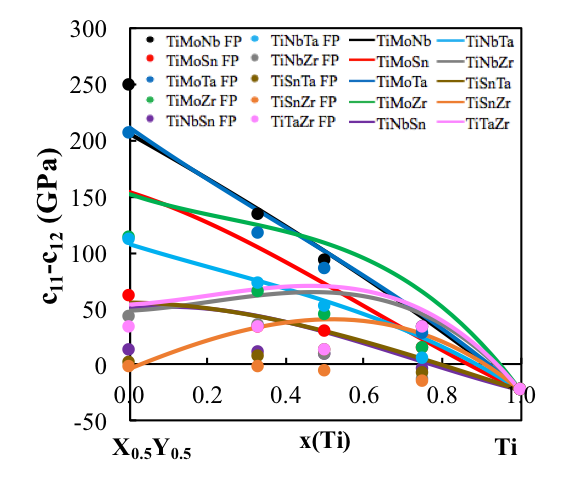
\includegraphics[width=\textwidth]{Chapter-6/Figures/tixyc11-c12.png}
	\caption{Calculated $\overline{C}_{11}$-$\overline{C}_{12}$ values (circles) plotted with the present modeling (solid lines) for the Ti-X-Y ternary systems (X $\neq$ Y = Mo, Nb, Ta, Sn, Zr). The $\overline{C}_{11}$-$\overline{C}_{12}$ shows the stability of the bcc phase, when the value is negative the bcc phase is not stable in the corresponding composition ranges.}
	\label{Ch6-figure:tixyc11-c12}
\end{figure}

\pagebreak
\begin{figure}[H]
	\centering
	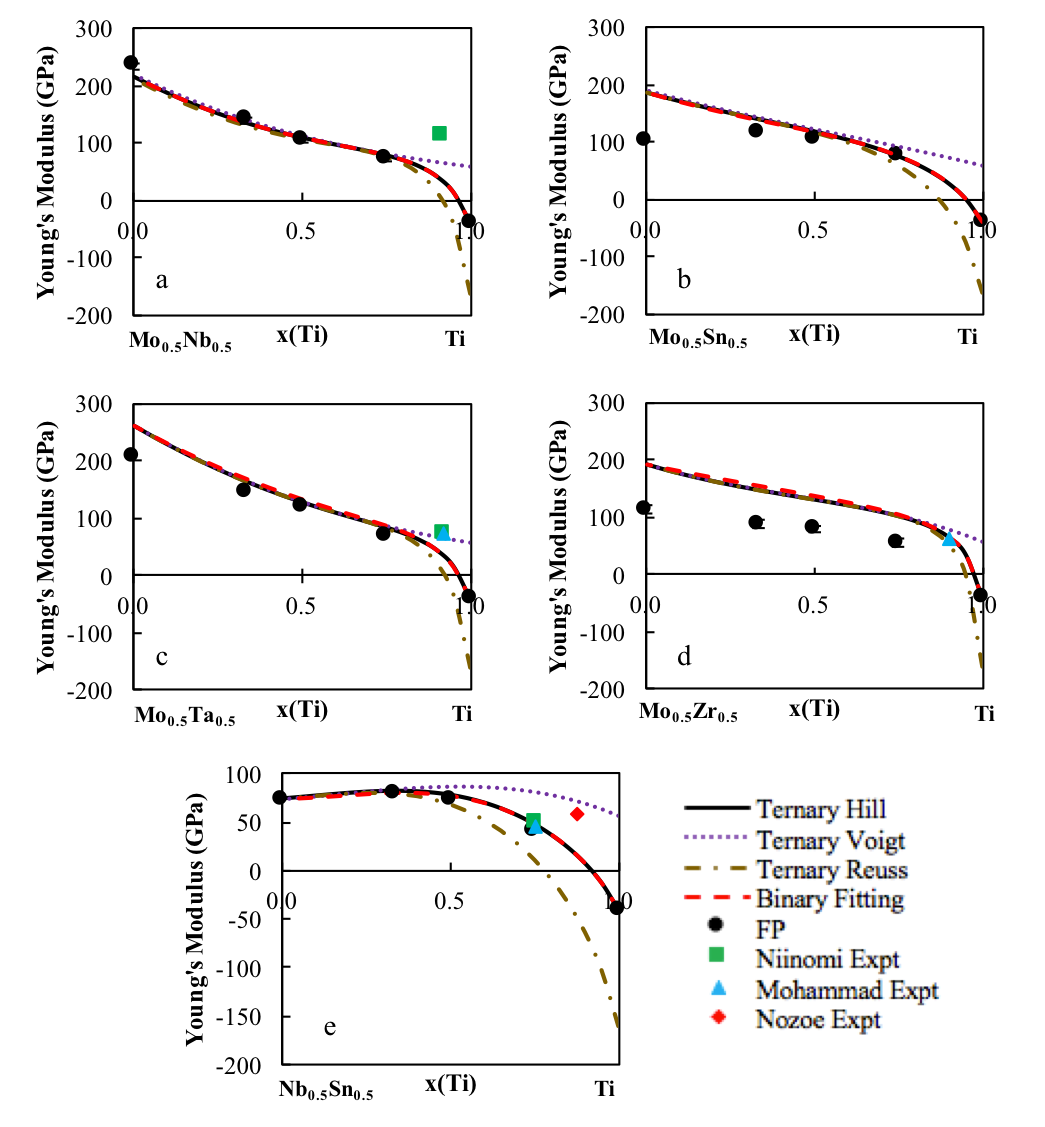
\includegraphics[width=\textwidth]{Chapter-6/Figures/tixyyoungs1.png}
	\caption{$E$ of five of the Ti-X-Y ternary systems are plotted from a 50-50 mixture of the alloying elements to Ti in the bcc phase. The present calculations are plotted as filled circles with the error bars. The red dotted line is the extrapolation for the pure elements and binary interaction parameters only. The dotted purple line is the Voigt upper $E$ bound, the gold dot dashed line is the lower Reuss $E$ bound and the black line is the Hill $E$ average. Experimental values are include for comparison \cite{Niinomi2012,Mohammed2014,Nozoe2007,Geetha2009}.}
	\label{Ch6-figure:tixyyoungs1}
\end{figure}

\pagebreak
\begin{figure}[H]
	\centering
	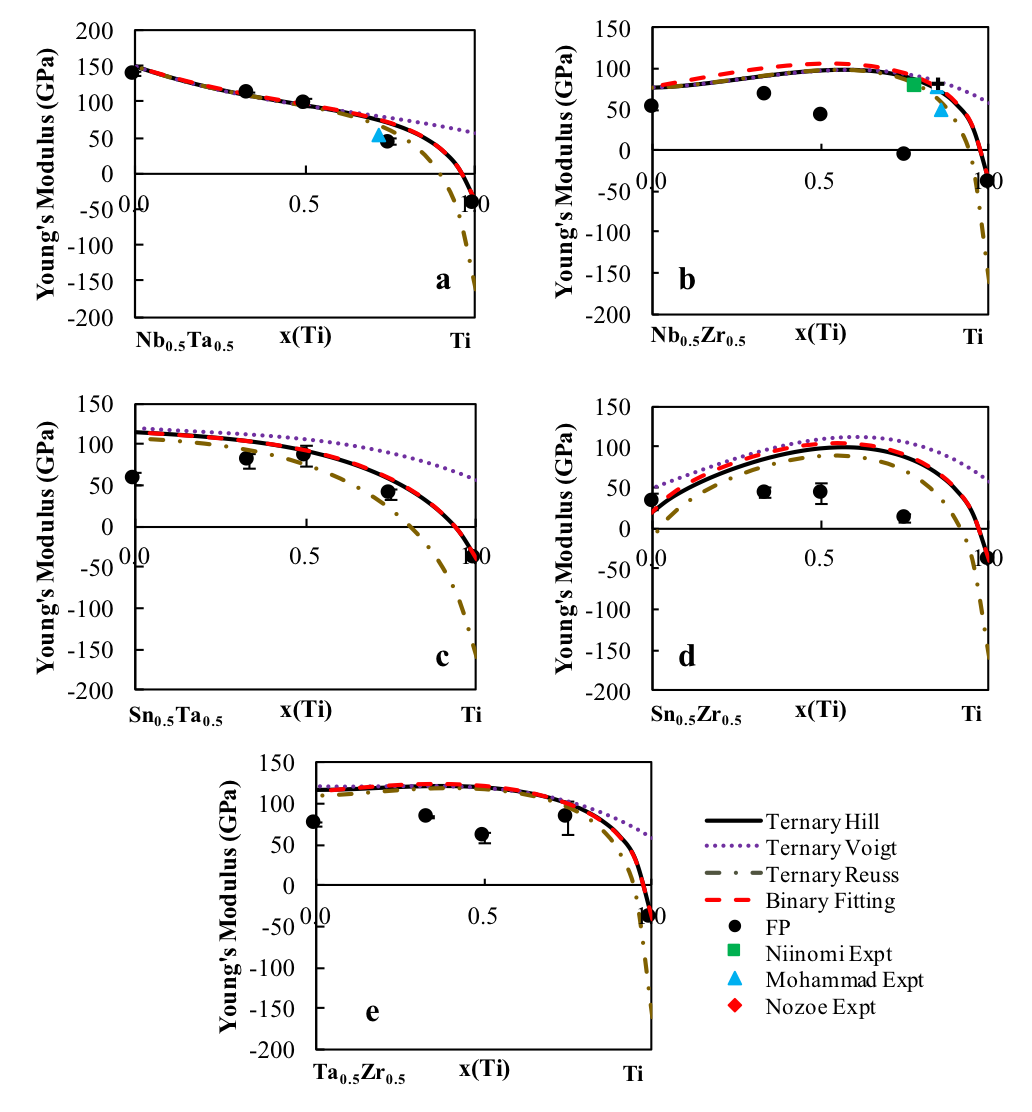
\includegraphics[width=\textwidth]{Chapter-6/Figures/tixyyoungs2.png}
	\caption{$E$ of five of the Ti-X-Y ternary systems are plotted from a 50-50 mixture of the alloying elements to Ti in the bcc phase. The present calculations are plotted as filled circles with the error bars. The red dotted line is the extrapolation for the pure elements and binary interaction parameters only. The dotted purple line is the Voigt upper $E$ bound, the gold dot dashed line is the lower Reuss $E$ bound and the black line is the Hill $E$ average. Experimental values are include for comparison \cite{Niinomi2012,Mohammed2014,Nozoe2007,Geetha2009}.}
	\label{Ch6-figure:tixyyoungs2}
\end{figure}

\pagebreak
\begin{figure}[H]
	\centering
	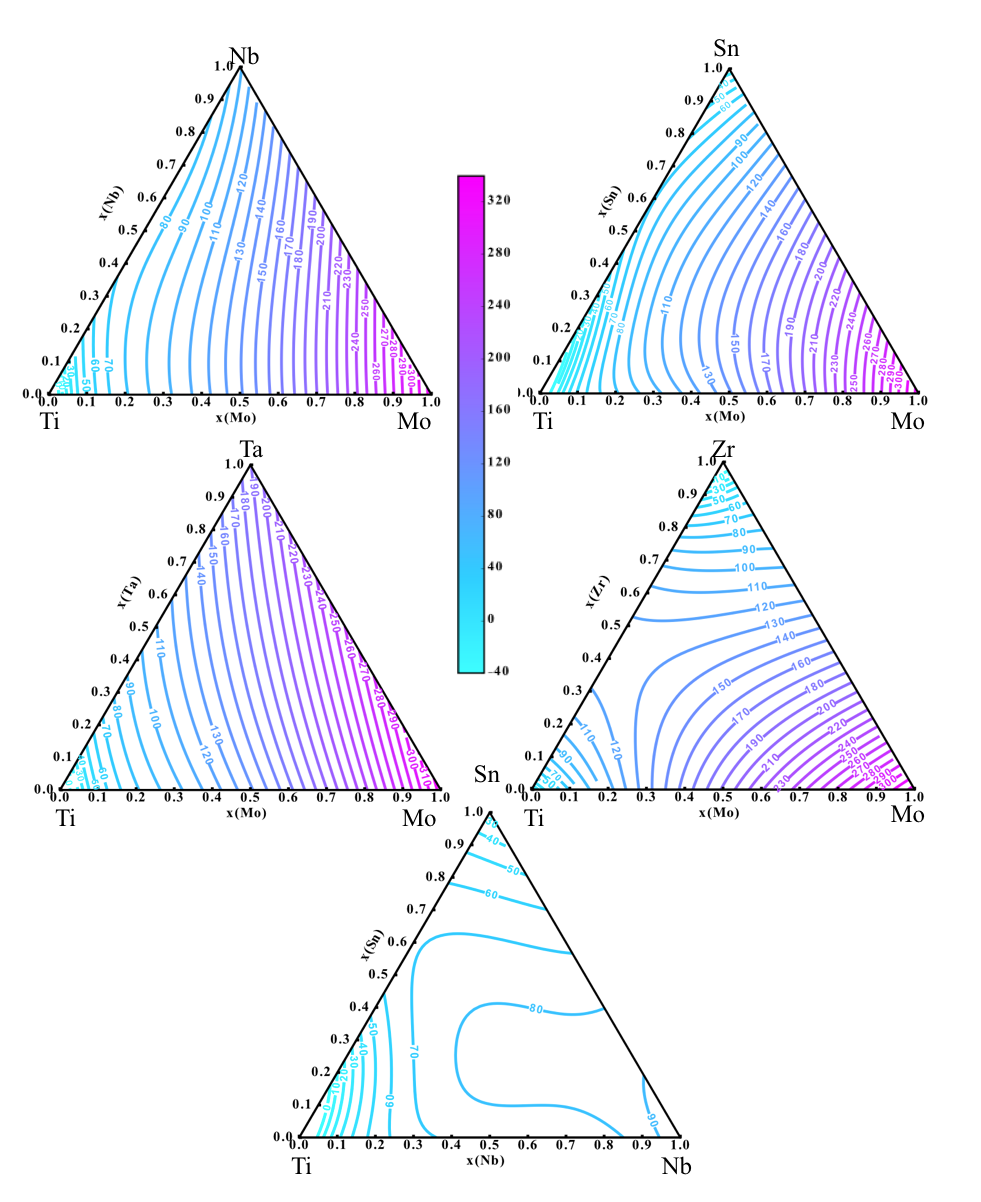
\includegraphics[width=\textwidth]{Chapter-6/Figures/tixymap1.png}
	\caption{The Young's modulus is mapped as a function of composition in GPa for the Ti-Mo-Nb, Ti-Mo-Sn, Ti-Mo-Ta, Ti-Mo-Zr and Ti-Nb-Sn alloy systems using pycalphad \cite{Otis2017}.}
	\label{Ch6-figure:tixymap1}
\end{figure}

\pagebreak
\begin{figure}[H]
	\centering
	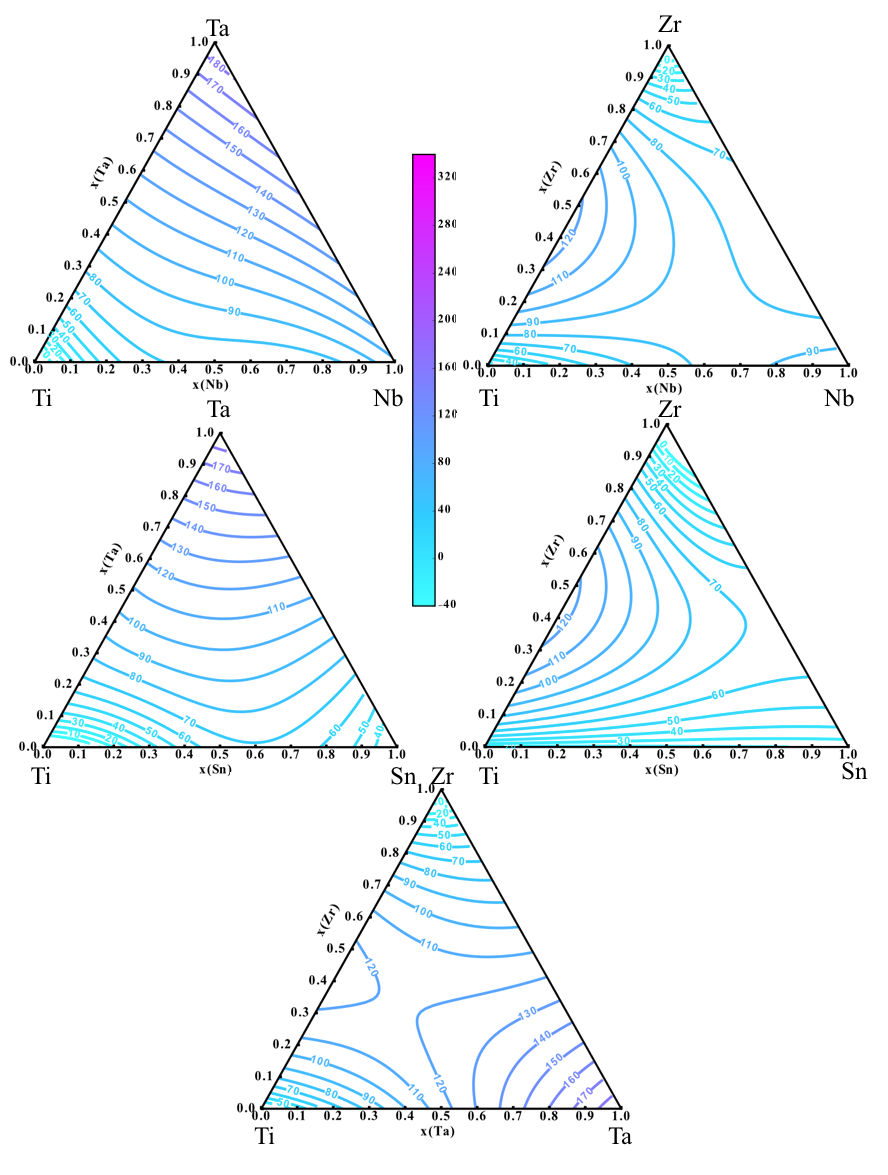
\includegraphics[width=\textwidth]{Chapter-6/Figures/tixymap2.png}
	\caption{The Young's modulus is mapped as a function of composition in GPa for the Ti-Mo-Nb, Ti-Mo-Sn, Ti-Mo-Ta, Ti-Mo-Zr and Ti-Nb-Sn alloy systems using pycalphad \cite{Otis2017}.}
	\label{Ch6-figure:tixymap2}
\end{figure}

\pagebreak
\begin{figure}[H]
	\centering
	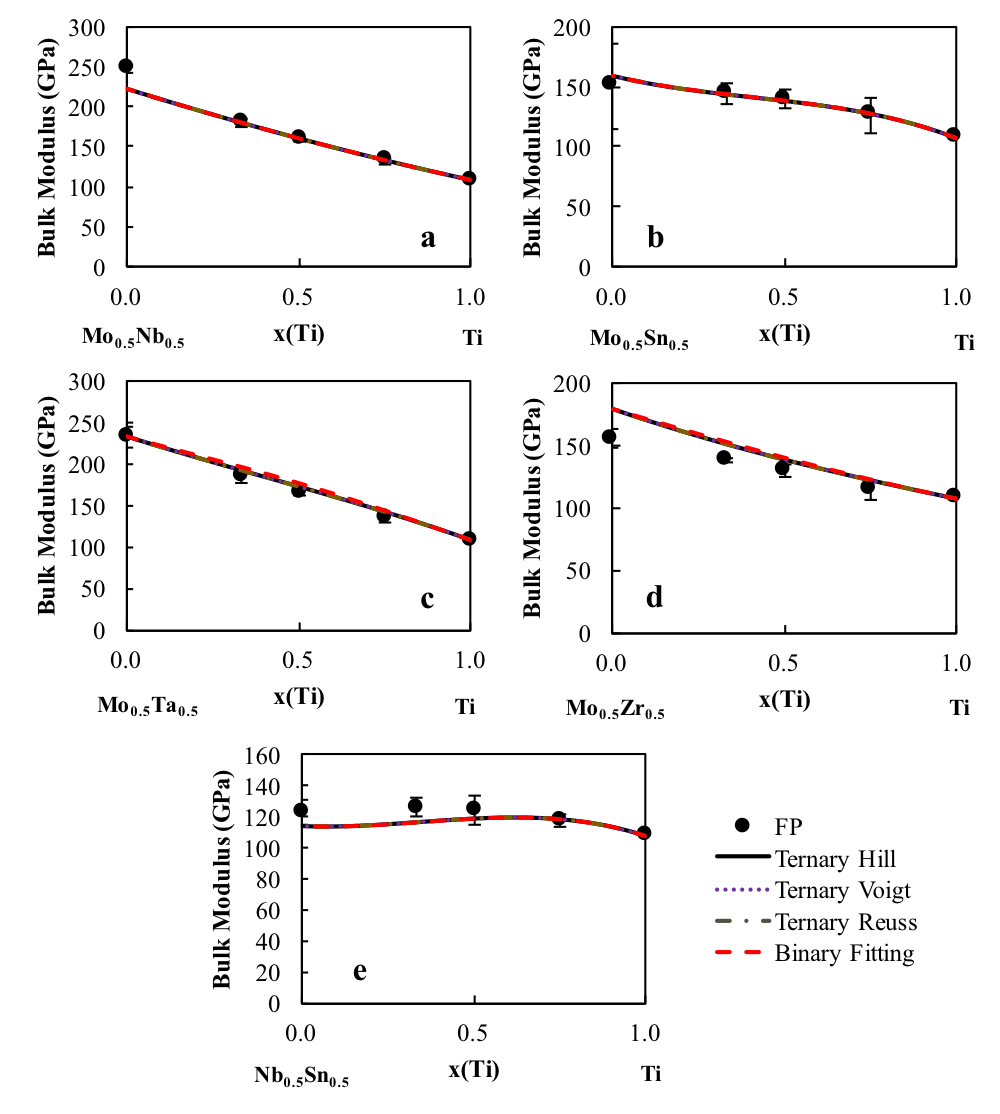
\includegraphics[width=\textwidth]{Chapter-6/Figures/tixybulk1.png}
	\caption{$B$ calculations of five of the Ti-X-Y ternary systems (X $\neq$ Y = Mo, Nb, Ta, Sn, Zr). The present calculations are plotted as the filled circles with error bars as well as the interpolation from the binary interaction parameters (red dashed line). The dotted purple line is the Voigt upper bulk modulus bound, the gold dashed line is the lower Reuss bulk modulus bound and the black line is the Hill bulk modulus average plotted from a 50-50 mixture of the alloying elements X and Y to Ti.}
	\label{Ch6-figure:tixybulk1}
\end{figure}

\pagebreak
\begin{figure}[H]
	\centering
	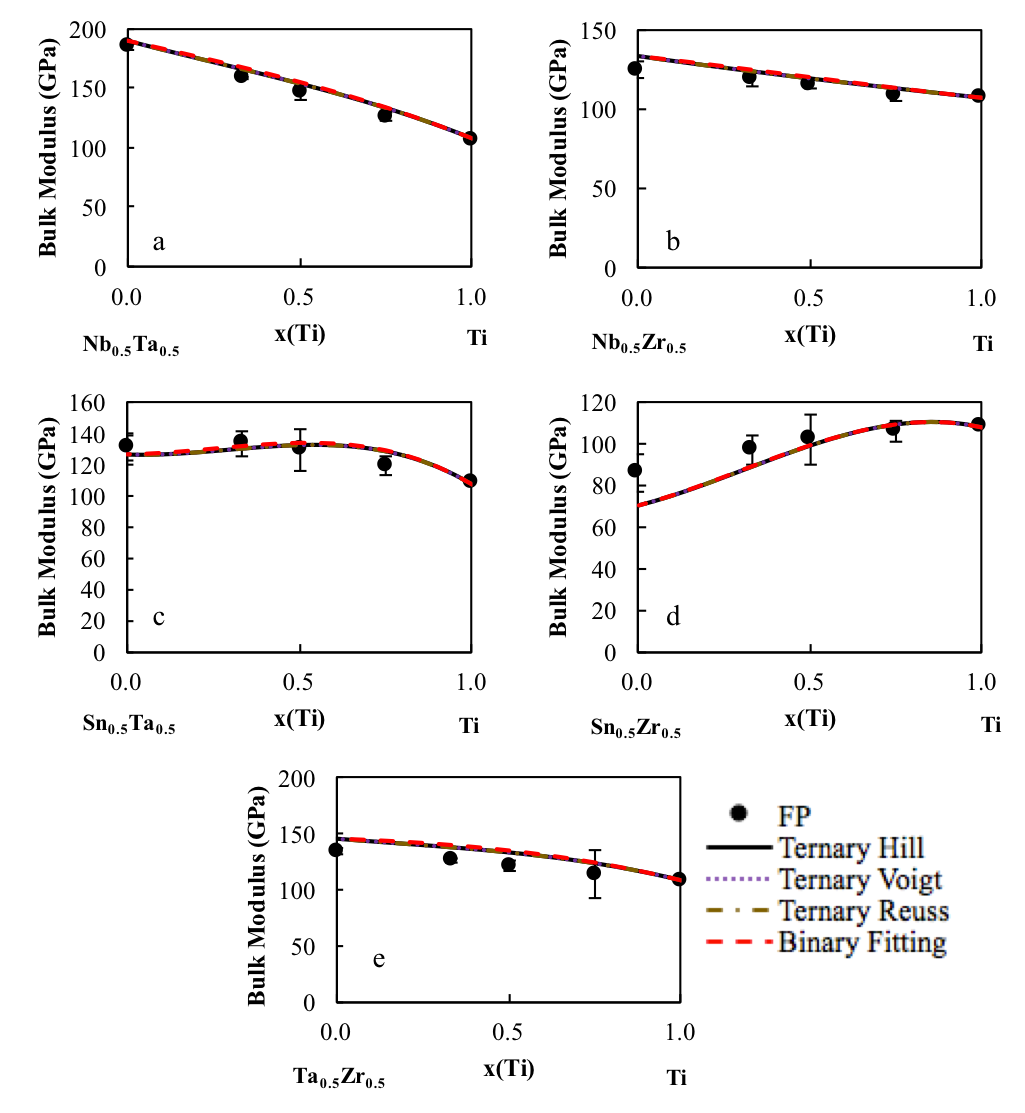
\includegraphics[width=\textwidth]{Chapter-6/Figures/tixybulk2.png}
	\caption{$B$ calculations of five of the Ti-X-Y ternary systems (X $\neq$ Y = Mo, Nb, Ta, Sn, Zr). The present calculations are plotted as the filled circles with error bars as well as the interpolation from the binary interaction parameters (red dashed line). The dotted purple line is the Voigt upper bulk modulus bound, the gold dashed line is the lower Reuss bulk modulus bound and the black line is the Hill bulk modulus average plotted from a 50-50 mixture of the alloying elements X and Y to Ti.}
	\label{Ch6-figure:tixybulk2}
\end{figure}

\pagebreak
\begin{figure}[H]
	\centering
	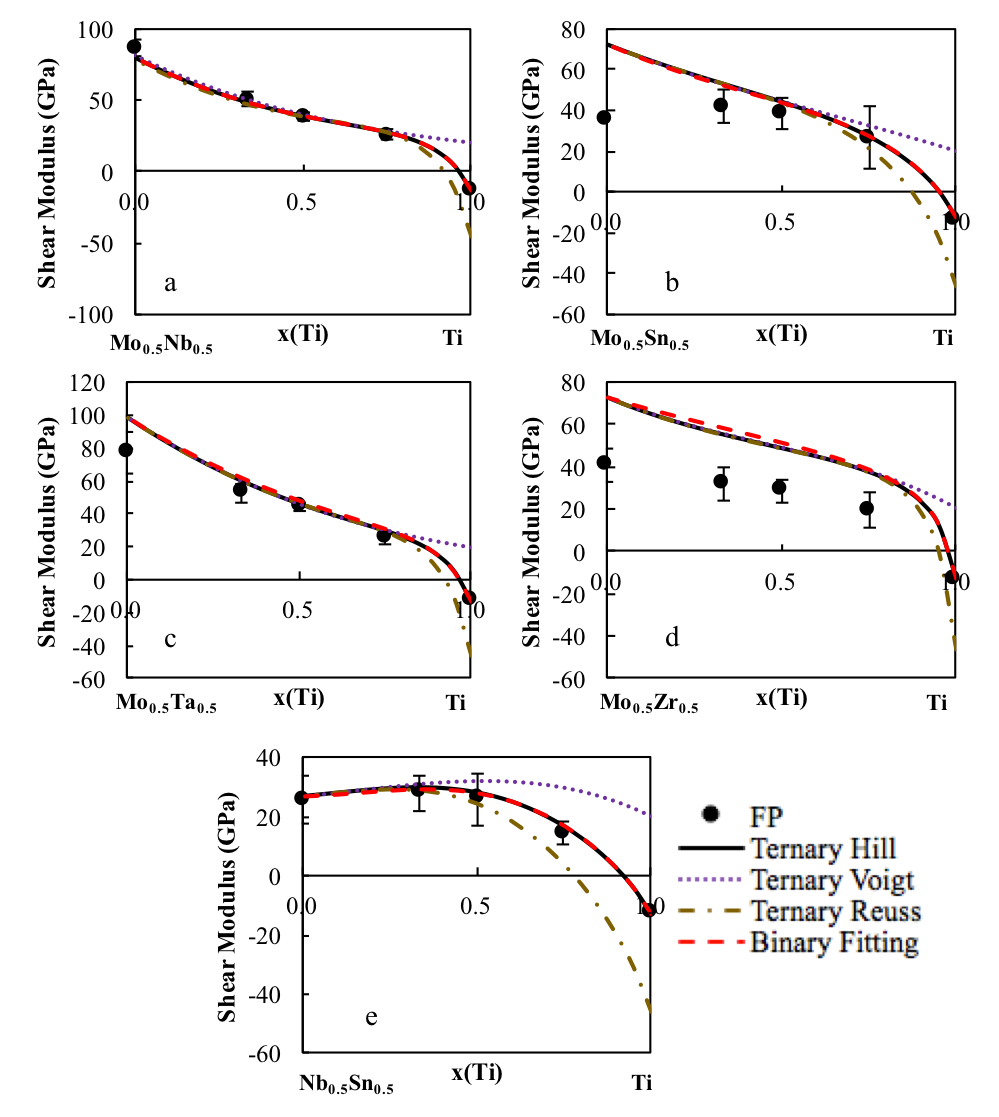
\includegraphics[width=\textwidth]{Chapter-6/Figures/tixyshear1.png}
	\caption{$G$ calculations of five of the Ti-X-Y ternary systems (X $\neq$ Y = Mo, Nb, Ta, Sn, Zr). The present calculations are plotted as the filled circles with error bars as well as the interpolation from the binary interaction parameters (red dashed line). The dotted purple line is the Voigt upper shear modulus bound, the gold dashed line is the lower Reuss shear modulus bound and the black line is the Hill shear modulus average plotted from a 50-50 mixture of the alloying elements X and Y to Ti.}
	\label{Ch6-figure:tixyshear1}
\end{figure}

\pagebreak
\begin{figure}[H]
	\centering
	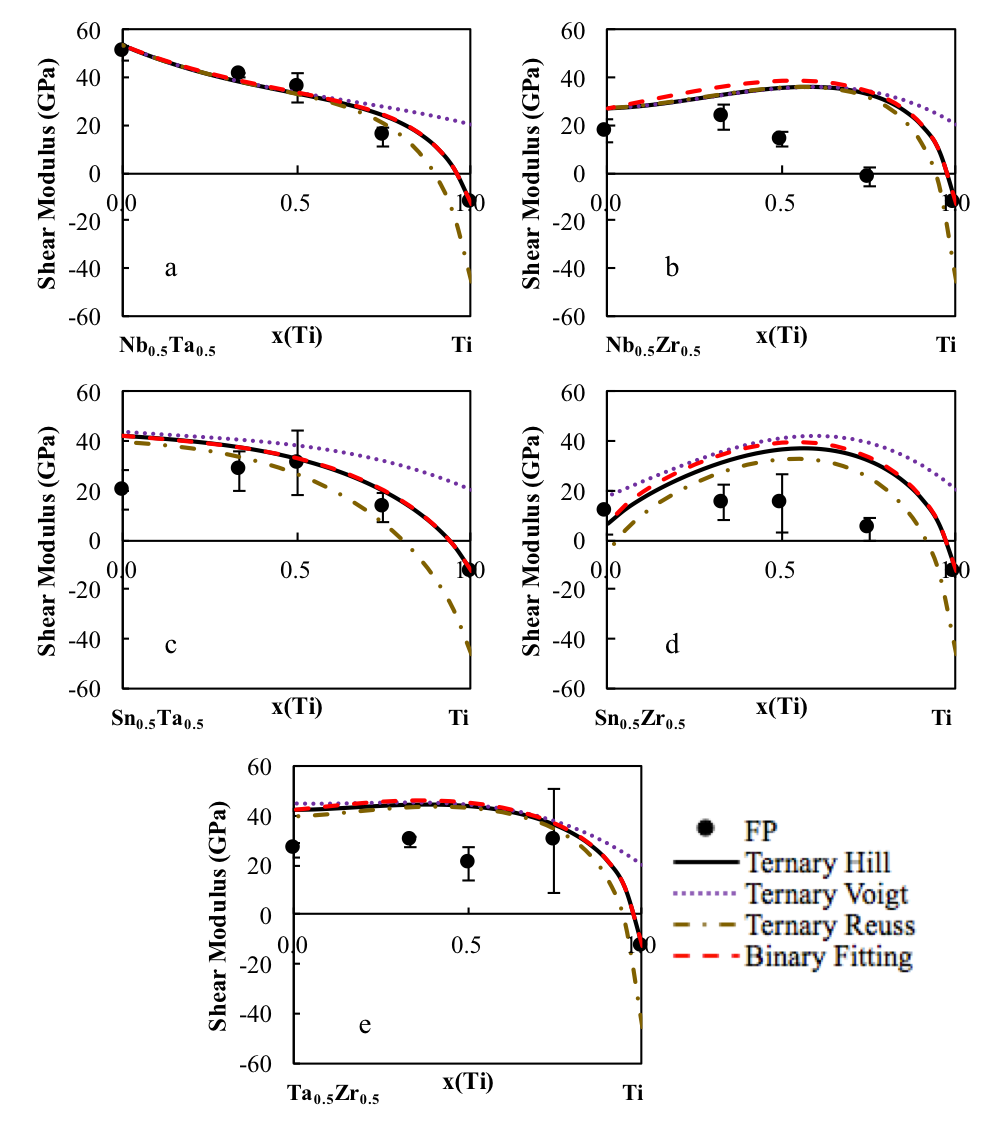
\includegraphics[width=\textwidth]{Chapter-6/Figures/tixyshear2.png}
	\caption{$G$ calculations of five of the Ti-X-Y ternary systems (X $\neq$ Y = Mo, Nb, Ta, Sn, Zr). The present calculations are plotted as the filled circles with error bars as well as the interpolation from the binary interaction parameters (red dashed line). The dotted purple line is the Voigt upper shear modulus bound, the gold dashed line is the lower Reuss shear modulus bound and the black line is the Hill shear modulus average plotted from a 50-50 mixture of the alloying elements X and Y to Ti.}
	\label{Ch6-figure:tixyshear2}
\end{figure}

\pagebreak
\begin{figure}[H]
	\centering
	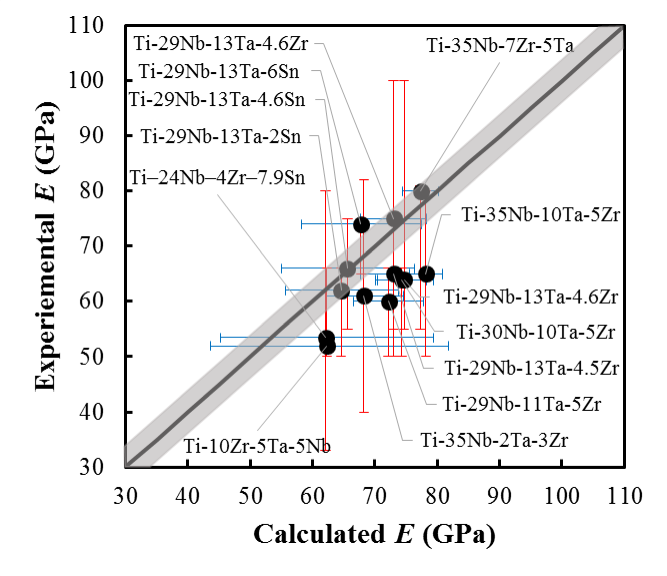
\includegraphics{Chapter-6/Figures/tixydatabase.png}
	\caption{$E$ of multicomponent bcc Ti alloys predicted from the database are compared with measured experimental results. Error bars plotted are from the variation in experimentally determined Young's moduli values for the specific multi-component alloy. The grey region refers to the error in the first-principles calculations. More information on the alloys is Table \ref{Ch6-table:tixydatacomp} \cite{Mohammed2014,Geetha2009,Tane2010a}.}
	\label{Ch6-figure:tixydatabase}
\end{figure}